% =============================================================================
%  重大活动交通态势洞察及辅助决策智能体集群 — LaTeX 模板
% =============================================================================
%  编译方式：
%      xelatex report.tex         （推荐，依赖 ctex + 系统字体）
%      latexmk -xelatex report.tex
%
%  字体准备（任选其一）：
%      • macOS:   Source Han Serif / Source Han Sans / Source Han Mono（系统自带或 Adobe）
%      • Linux:   Noto Serif CJK SC / Noto Sans CJK SC / Noto Sans Mono CJK SC
%      • Windows: SimSun / SimHei（仅作演示）
%
%  说明：
%      1. 本模板保留了 Markdown 原稿的章节结构与排版风格；
%      2. 各章节内含示例文本，便于编译后直接核对样式；
%      3. 表格、提示框、代码块、图片均已封装为可直接复用的命令/环境。
% =============================================================================

\documentclass[a4paper,11pt]{article}

% -----------------------------------------------------------------------------
%  中文与字体
%  根据本地可用字体调整 \setmainfont / \setCJKmainfont 等命令：
%    • macOS:   STSong（宋体）/ STHeiti（黑体）/ STFangsong（仿宋）/ PingFang SC
%    • Linux:   Noto Serif CJK SC / Noto Sans CJK SC
%    • Windows: SimSun / SimHei / Microsoft YaHei
% -----------------------------------------------------------------------------
\usepackage[UTF8,fontset=none]{ctex}
% 西文（TeX Live 自带 TeX Gyre，无需额外安装）
\setmainfont{texgyretermes-regular.otf}[
  BoldFont       = texgyretermes-bold.otf,
  ItalicFont     = texgyretermes-italic.otf,
  BoldItalicFont = texgyretermes-bolditalic.otf,
]
\setsansfont{texgyreheros-regular.otf}[
  BoldFont       = texgyreheros-bold.otf,
  ItalicFont     = texgyreheros-italic.otf,
  BoldItalicFont = texgyreheros-bolditalic.otf,
]
\setmonofont{texgyrecursor-regular.otf}[
  BoldFont       = texgyrecursor-bold.otf,
  ItalicFont     = texgyrecursor-italic.otf,
  BoldItalicFont = texgyrecursor-bolditalic.otf,
]
% 中文（macOS 系统字体；若为 Linux/Windows 请按上方注释替换）
%   \setCJKmainfont 不指定 BoldFont：使用 ctex 内部 BoldFont 映射以避免未安装字体报警
\setCJKmainfont{STSong}
\setCJKsansfont{STHeiti}
\setCJKmonofont{STFangsong}
% 如果需要获得更丰富的字重，可改为在主字体使用独立的 Bold 字体（要求系统已安装）
% \setCJKfamilyfont{cjkbold}{STHeiti}

% -----------------------------------------------------------------------------
%  页面布局
% -----------------------------------------------------------------------------
\usepackage[a4paper,top=2.5cm,bottom=2.5cm,left=2.5cm,right=2.5cm]{geometry}
\usepackage{indentfirst}      % 中文首行缩进
\setlength{\parindent}{2em}  % 中文段落标准缩进 2 字
\linespread{1.3}             % 1.3 倍行距，接近 Markdown 渲染密度

% -----------------------------------------------------------------------------
%  颜色与图形
% -----------------------------------------------------------------------------
\usepackage{xcolor}
\usepackage{colortbl}
\usepackage{graphicx}
\graphicspath{{./}{./assets/}{./assets/重大活动交通态势洞察及辅助决策智能体集群/}}

% TikZ（技术架构图）
\usepackage{tikz}
\usetikzlibrary{positioning, shapes.geometric, arrows.meta, fit, backgrounds, calc, shadows.blur}

% 报告用色
\definecolor{ImportantColor}{RGB}{180,40,40}
\definecolor{WarningColor}{RGB}{200,140,0}
\definecolor{CautionColor}{RGB}{210,80,30}
\definecolor{TipColor}{RGB}{40,110,180}
\definecolor{NoteColor}{RGB}{90,90,90}
\definecolor{TableHead}{RGB}{230,235,240}

% -----------------------------------------------------------------------------
%  表格
% -----------------------------------------------------------------------------
\usepackage{booktabs}
\usepackage{tabularx}
\usepackage{array}
\usepackage{longtable}
\usepackage{multirow}
\renewcommand{\arraystretch}{1.25}  % 表格行高

% -----------------------------------------------------------------------------
%  列表
% -----------------------------------------------------------------------------
\usepackage{enumitem}
\setlist[itemize]{leftmargin=1.5em,topsep=2pt,parsep=1pt,itemsep=2pt}
\setlist[enumerate]{leftmargin=1.8em,topsep=2pt,parsep=1pt,itemsep=2pt}

% -----------------------------------------------------------------------------
%  代码块
% -----------------------------------------------------------------------------
\usepackage{listings}
\lstset{
  basicstyle=\ttfamily\small,
  breaklines=true,
  columns=fullflexible,
  frame=single,
  framerule=0.4pt,
  framesep=4pt,
  xleftmargin=1em,
  xrightmargin=1em,
  aboveskip=8pt,
  belowskip=8pt,
}

% -----------------------------------------------------------------------------
%  提示框（对应 Markdown 的 [!IMPORTANT] / [!WARNING] / [!TIP] / [!CAUTION] / 引用块）
% -----------------------------------------------------------------------------
\usepackage[most]{tcolorbox}

% 通用提示框
\newtcolorbox{admonition}[2]{
  enhanced, breakable,
  colback=#1!5!white,
  colframe=#1!75!black,
  fonttitle=\bfseries\sffamily,
  title={#2},
  boxrule=0.6pt, arc=2pt,
  left=8pt, right=8pt, top=4pt, bottom=4pt,
  before skip=8pt, after skip=8pt,
}

% 派生环境（直接使用即可，无需参数）
\newenvironment{important}{\begin{admonition}{ImportantColor}{重要提示}}{\end{admonition}}
\newenvironment{warning} {\begin{admonition}{WarningColor} {警告提示}}{\end{admonition}}
\newenvironment{tip}     {\begin{admonition}{TipColor}     {操作提示}}{\end{admonition}}
\newenvironment{caution} {\begin{admonition}{CautionColor} {注意事项}}{\end{admonition}}
\newenvironment{note}    {\begin{admonition}{NoteColor}    {备注}    }{\end{admonition}}

% 引用块（Markdown 中的 `> ...`）
\newenvironment{quoteblock}{%
  \begin{tcolorbox}[
    enhanced, breakable,
    colback=gray!5!white,
    colframe=gray!50!black,
    boxrule=0.4pt, arc=2pt,
    left=8pt, right=8pt, top=4pt, bottom=4pt,
    before skip=6pt, after skip=6pt,
  ]\itshape
}{\end{tcolorbox}}

% -----------------------------------------------------------------------------
%  超链接与书签
% -----------------------------------------------------------------------------
\usepackage[colorlinks=true,
            linkcolor=blue!60!black,
            urlcolor=blue!60!black,
            citecolor=blue!60!black,
            bookmarksnumbered=true,
            bookmarksopen=true]{hyperref}

% -----------------------------------------------------------------------------
%  标题格式
% -----------------------------------------------------------------------------
\usepackage{titlesec}
\titleformat{\section}{\Large\bfseries\sffamily}{\thesection}{1em}{}
\titleformat{\subsection}{\large\bfseries\sffamily}{\thesubsection}{1em}{}
\titleformat{\subsubsection}{\normalsize\bfseries\sffamily}{\thesubsubsection}{1em}{}
\titlespacing*{\section}      {0pt}{2.5ex plus 1ex minus .2ex}{1.5ex plus .2ex}
\titlespacing*{\subsection}   {0pt}{2.0ex plus 1ex minus .2ex}{1.0ex plus .2ex}
\titlespacing*{\subsubsection}{0pt}{1.5ex plus 1ex minus .2ex}{0.8ex plus .2ex}

% -----------------------------------------------------------------------------
%  目录样式
% -----------------------------------------------------------------------------
\usepackage{tocloft}
\renewcommand{\cfttoctitlefont}{\Large\bfseries\sffamily}
\renewcommand{\cftsecfont}{\sffamily}
\renewcommand{\cftsecpagefont}{\normalfont}
\renewcommand{\cftsubsecfont}{\sffamily}
\renewcommand{\cftsubsubsecfont}{\sffamily}
\setlength{\cftbeforesecskip}{4pt}
\setlength{\cftbeforesubsecskip}{2pt}

% -----------------------------------------------------------------------------
%  页眉页脚
% -----------------------------------------------------------------------------
\usepackage{fancyhdr}
\pagestyle{fancy}
\fancyhf{}
\fancyhead[L]{\small\sffamily 重大活动交通态势洞察及辅助决策智能体集群}
\fancyhead[R]{\small\sffamily v2.14.0}
\fancyfoot[C]{\thepage}
\renewcommand{\headrulewidth}{0.4pt}

% -----------------------------------------------------------------------------
%  杂项命令
% -----------------------------------------------------------------------------
% 元信息行（项目表用）
\newcommand{\metarow}[2]{\textbf{#1} & #2 \\}
% 代码片段
\newcommand{\code}[1]{\texttt{#1}}
% 段中强调
\newcommand{\term}[1]{\textbf{#1}}

% 图片：默认在 assets/重大活动交通态势洞察及辅助决策智能体集群/ 下查找。
% 如需使用其他目录，请修改 \graphicspath 或直接传完整路径给 \includegraphics。
\newcommand{\reportimg}[2][]{%
  \begin{figure}[ht]
    \centering
    \includegraphics[width=0.92\linewidth]{#2}
    \ifx&#1&\else \caption*{#1}\fi
  \end{figure}%
}

% =============================================================================
%  文档开始
% =============================================================================
\begin{document}

% -----------------------------------------------------------------------------
%  标题页
% -----------------------------------------------------------------------------
\begin{titlepage}
\centering
\vspace*{2cm}

{\sffamily\bfseries\Huge 重大活动交通态势洞察\\[0.4em]及辅助决策智能体集群}\\[2.5em]
{\Large\bfseries\sffamily 项目建设说明报告}\\[1em]
{\large\sffamily Project Build Report}\\[6em]

\rule{0.55\linewidth}{0.5pt}\\[2.5em]

\begin{tabularx}{0.78\linewidth}{@{}lX@{}}
\toprule
\rowcolor{TableHead}
\multicolumn{2}{@{}l}{\sffamily\bfseries 项目元信息} \\
\midrule
\metarow{系统名称}{TransportX Agent Workshop}
\metarow{当前版本}{v2.14.0}
\metarow{案例对象}{2025 年 8 月上海体育场重大活动}
\metarow{编制日期}{2026 年 7 月 30 日}
\metarow{文档状态}{完善稿，以本 Markdown 文件为准}
\bottomrule
\end{tabularx}

\vfill

{\small\sffamily 本报告依据仓库实现、数据资产说明、知识库索引和自动化测试结果编制。\\工程测试用于核查系统功能与安全边界。\\问数准确率和方案采纳率需单独开展业务验收。}

\vspace{1cm}
\end{titlepage}

% -----------------------------------------------------------------------------
%  摘要
% -----------------------------------------------------------------------------
\section*{摘要}
\addcontentsline{toc}{section}{摘要}

重大活动交通保障数据分散在多个文件和系统中，各类数据的统计口径也有差异。分析人员完成一次研判，通常需要在数据库、制图工具和报告之间多次转录。本项目为此开发了浏览器端智能体工作台，将数据治理、外部数据接入、知识检索、交通问数、任务编排、地图和报告放在同一套系统中。当前案例选取上海体育场四场演唱会，使用公交、轨交、道路、网约车和气象数据，并接入 EVDATA 新能源汽车数据服务获取道路速度和实时路况。

项目名称中的``智能体集群''指由同一智能体统一调用的能力集合。智能体根据任务使用数据问数、决策辅助、任务控制、知识检索、地图呈现和报告生成等能力。各项能力由明确的工具与 Skill 约束，数据库权限、文件范围、地图渲染和引用来源由程序控制。

% -----------------------------------------------------------------------------
%  目录
% -----------------------------------------------------------------------------
\newpage
\tableofcontents

% =============================================================================
%  一、总体概述
% =============================================================================
\newpage
\section{总体概述}

\subsection{建设目标与定位}

本项目服务重大活动交通态势研判和保障决策。业务人员用自然语言提出问题，工作台查询授权范围内的数据，完成对比、制图和报告整理。每次任务保存数据来源、执行步骤和结果文件，复核时可以沿原路径回查。

系统用于分析辅助，指挥和审批仍由交通管理部门负责。活动前，业务人员可识别重点时段、站点和交通方式；活动期间，可查看已有数据反映的趋势和空间分布；活动结束后，可对比活动日与对照日，并保存查询和报告。

项目统一订单、端点、客流和道路状态的统计口径。系统以结构化数据保存查询过程、任务状态、地图场景和引用记录，分析结果可直接写入地图、表格和报告。

\subsection{场景描述与能力边界}

当前版本处理四类常见问题。原始数据分散在不同文件和坐标系中，同一订单容易重复统计；公交交易数、轨交人次、订单数和端点事件经常混用；查询、制图和报告之间存在重复转录；法规、预案和案例依据缺少稳定的引用位置。项目分别建立统一数据资产、只读查询接口、声明式地图和知识 ID。

当前版本覆盖五类业务场景。交通问数支持按日期、时段、线路、站点、道路发布段、订单方向等条件查询，并进行活动日与非活动日对比。空间分析发布经校验的 GeoJSON，绘制场馆、轨交网络、客流热点和重要枢纽，支持图层增量更新与选择交互。辅助研判按演前集结、演出中运行和散场疏散三个阶段整理证据，列出风险点、建议动作和待确认事项。知识检索与引用从法规、标准、预案、案例和项目资料中定位原文节点，登记可核查引用。成果交付则在同一会话中预览代码、表格、图片和 Markdown 报告，并将报告导出为 PDF。

\begin{important}
组织方提供的交通事实数据覆盖约 21--22 天，可用于活动期短周期对比。轨交客流覆盖 10 个物理站；原始道路数据含 89 个发布段，没有几何；天气网格坐标系待确认。EVDATA 接口可提供实时道路速度和路况，当前入库并验收的数据为 2025 年 8 月 24 日单日样本。季节性、年度趋势和持续实时分析需要更长时间的数据。封路、停运、限流、警力部署等措施由业务部门核实并按法定程序审批。
\end{important}

\subsection{核心成果亮点概述}

系统围绕交通保障业务，重点在五个方面构建能力。

在工作台内一站式开展交通分析。业务人员用自然语言提出问题即可在同一界面完成数据查询、任务跟踪、地图分析和报告整理，不再需要在数据库、制图工具和报告之间反复切换。

统一理解多源交通数据。公交、轨交、道路、网约车、气象和空间信息在时间、位置和统计口径上对齐，让不同来源的数据可以放在同一坐标系下对照，避免跨域比较时口径不一致。

直观呈现活动周边态势。客流变化、交通热点、轨交站点和重点场所直接落到地图上，便于快速识别重点时段和重点区域，也让分析结果可以通过图层显隐和叠加控制逐项核查。

为研判和方案提供依据。数据分析结果与法规、预案、标准和同类案例结合，生成建议时同步保留出处；业务人员在采纳前可以沿着引用条目回到原文核对，避免``黑盒推荐''。

保留完整的分析过程。每次任务使用的数据、步骤、地图和报告都保存在会话目录中，业务人员既能恢复历史任务，也能沿原过程复核结论。

% =============================================================================
%  二、总体技术架构
% =============================================================================
\newpage
\section{总体技术架构}

\subsection{总体架构设计}

系统面向交通管理、运营和分析人员，围绕``提出问题、查看态势、研判方案''组织能力。整体架构由统一工作台、智能体能力协同、受控能力和支撑资源四个部分组成。业务人员通过一个入口完成提问、任务跟踪、地图查看和成果确认，智能体根据任务调用数据、知识和分析工具。

\begin{figure}[ht]
  \centering
  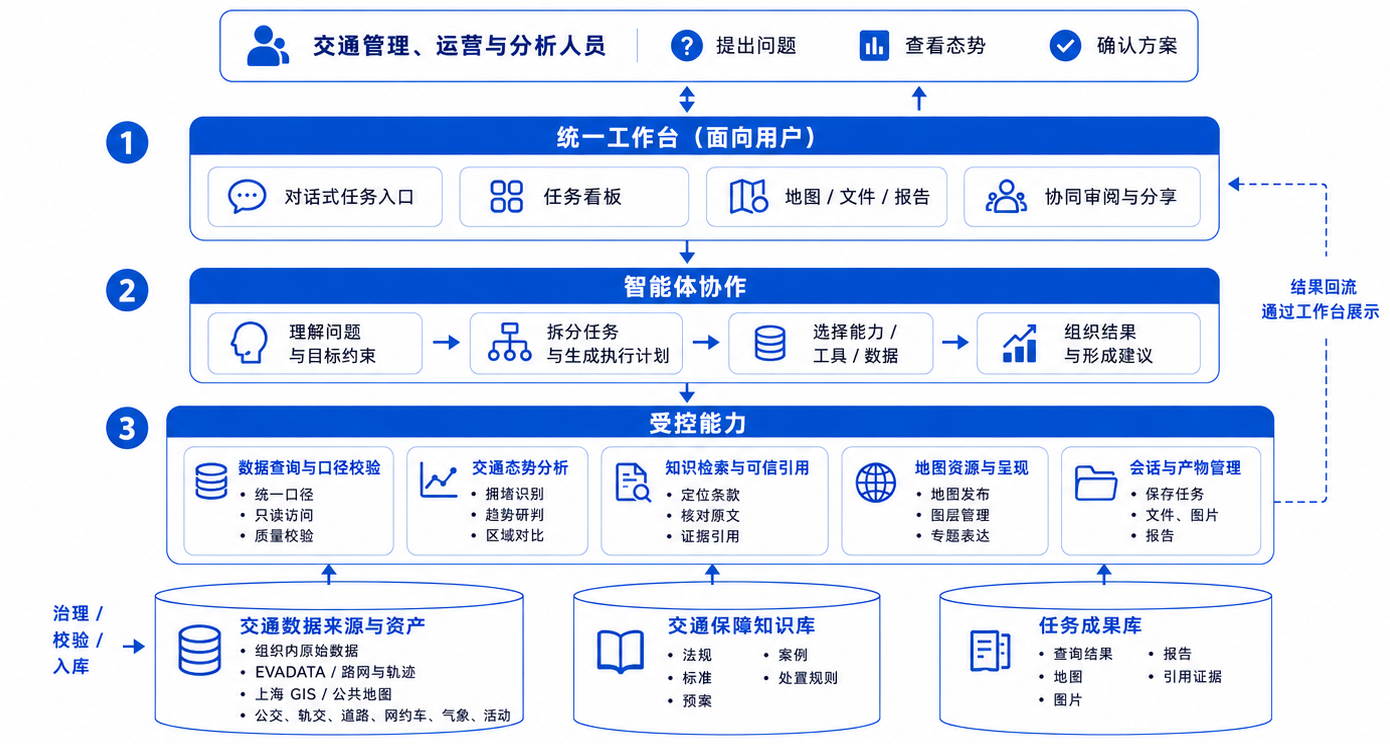
\includegraphics[width=0.92\linewidth]{00-overall-architecture.png}
  \caption{重大活动交通态势洞察及辅助决策智能体集群总体架构}
  \label{fig:architecture}
\end{figure}

图中自上而下展示了完整工作路径。图中的``智能体协作''表示同一智能体内部的多种能力协同。工作台承接业务人员的操作，智能体负责理解问题和组织任务，受控能力完成查询、分析、引用和成果管理，底层资源提供交通数据、保障知识和任务文件。分析结果返回工作台后，业务人员可以继续追问、调整任务或确认方案。

\subsection{分层模块说明}

\subsubsection{统一工作台}

统一工作台是业务人员使用系统的入口，集中承载对话、任务看板、地图、文件和报告。用户可以在同一界面提出交通问题、查看处理进度、核对空间分布并整理成果。不同会话和任务分别保存，历史分析可以恢复和继续。

\subsubsection{智能体能力协同}

智能体能力协同层负责把业务问题转化为可执行任务。同一智能体围绕当前任务按需调用四类能力：先做问题理解与口径确认，识别活动、日期、时段、区域、交通方式和指标，发现歧义时向用户确认；再进入任务规划与过程管理，把复杂问题拆分为可检查的步骤并跟踪执行进度、保留中间结果；然后通过数据查询与态势分析比较不同日期、时段、区域和交通方式，识别趋势、热点和异常；最后结合法规、预案、标准和案例完成知识检索与辅助研判，整理风险、建议措施和待确认事项。这些能力共享同一任务上下文，按分析需要依次调用，状态、数据结果和地图资源按会话隔离。

\subsubsection{受控能力}

受控能力层负责执行具体操作。数据查询按照已登记的表、字段和指标口径运行；态势分析使用统一的时间和空间规则；知识检索保留文档、条款和原件位置；地图展示只接收经过校验的空间数据；文件和报告按任务目录保存。

这一层把智能体提出的操作转化为明确的查询、分析和发布动作。数据库保持只读，地图命令、文件路径和引用来源均受规则约束，任务过程可以检查和回放。

\subsubsection{支撑资源}

底层资源分为三类。交通数据来源与资产涵盖组织方原始数据、EVDATA 道路数据、上海 GIS 与公开地图补充信息，以及治理形成的公交、轨交、道路、网约车和气象数据资产。交通保障知识库汇集法规、标准、预案、案例和项目资料，为措施研判和报告引用提供依据。任务成果包括查询结果、地图、图片、引用和报告，随任务保存在工作台目录，可供查看、下载和复核。

\subsection{核心技术选型清单}

\begin{itemize}
  \item \term{智能体运行时：}本项目在 Coding Agent 0.80.10 之上自研轻量级 Agent Loop，统一管理单会话内的多轮工具调用与任务步骤管理。Loop 围绕“问题理解—工具调用—结果整理”循环设计，结构简洁、按需装配，便于在受控环境下稳定运行；模型可配置，支持会话恢复、工具契约、单步签与排队控制。
  \item \term{服务端：}采用 Node.js、TypeScript 和 WebSocket，负责运行时进程、会话状态与受控资源管理。能力通过 Extension 注册，数据库、文件路径和地图命令受规则约束；运行时能力通过 RuntimeCapabilities 声明为共享契约。
  \item \term{前端工作台：}采用 React 19、Vite 8、Tailwind CSS 4 和 Radix Dialog，提供对话、任务看板、地图、文件和报告的响应式布局；通过命令面板与状态机引导任务模式，浏览器内核按契约渲染。
  \item \term{地图呈现：}采用 MapLibre GL 5.24 和 GeoScene v1，通过结构化命令更新图层、样式和视角；地图状态与会话一起持久化，便于复核；增量发布与白名单命令保障发布安全。
  \item \term{内容呈现：}采用 Markdown、Mermaid、KaTeX、Shiki 和 XLSX，支持报告、流程图、公式、代码与数据文件预览；通过相对路径安全校验后渲染。
  \item \term{数据存储与治理：}采用 6 个 SQLite 分域库和 Python 3.10 脚本，按“原始层→标准层→事实→集市”逐层派生；问数优先查询集市，错误级质量规则触发即阻断发布。
  \item \term{质量验证：}采用 node:test 与 Playwright 覆盖会话、鉴权、任务、地图、引用和浏览器交互；模拟运行时与真实运行时冒烟测试，70 项自动化测试全部通过。
\end{itemize}

% =============================================================================
%  三、数据接入与治理
% =============================================================================
\newpage
\section{数据接入与治理}

\subsection{基础数据}

组织方提供的原始业务数据位于 \code{data/徐汇区各业态数据}，共 9 个文件，其中 CSV 7 个、XLSX 2 个。Excel 工作表拆分后登记为 12 个逻辑数据集，共 2,524,322 条源记录。GIS 静态网络、EVDATA 数据、POI、活动日程、时间维度和治理派生表由项目后续补充。原始文件保存在外部受控目录，项目仓库只保存代码、说明和知识资产。所有业务时间按 \code{Asia/Shanghai} 解释。

网约车订单包含上车端点 641,134 行、下车端点 634,446 行，记录订单号、时间、经纬度和坐标系信息，用于订单趋势、OD 和空间热点分析；其中与场馆关联的离场订单约 57.9 万行、到场订单约 57.2 万行，用于补齐行程并识别场馆出入方向。公交数据由 55,339 条半小时客流记录和 75 条有客流线路构成，叠加 77 条官方线路、194 个官方站点和 652 条站序关系，客流用于线路趋势和活动日对比，静态数据用于实体匹配。轨交客流共 7,975 条线路—站点—小时记录，覆盖 10 个物理站，记录进出站人次用于站点和高峰时段分析。道路状态由 21,775 条``逢变更新''事件组成，覆盖 89 个发布段，用于还原各状态的持续时间。气象观测共 11,384 条记录，覆盖徐汇区 8 个网格，温度和降雨信息以分钟粒度提供；网格坐标系尚未确认，当前按网格名称和小时关联。

\begin{caution}
公交交易数、轨交进出站人次、网约车订单、端点事件和场馆事件使用不同量纲，分析时分别统计。15:00--19:00、19:00--22:00、22:00--24:00 为案例分析窗口。官方开门、演出和管控时刻以活动方案为准。
\end{caution}

\subsection{外部接入与项目补充数据}

3.1 列明的 9 个文件由组织方提供。其余数据来自外部接口、上海 GIS/公开地图资料、用户确认或程序派生，来源在资产目录中单独登记。这些数据补充道路动态、空间坐标、交通网络和分析所需的时空维度。

EVDATA 新能源汽车道路数据已通过接口接入，可获取实时路况；当前入库样本为 2025 年 8 月 24 日的 207 个 WGS84 路段和 14,977 条 15 分钟速度记录，用于道路速度趋势和空间分析；EVDATA 路段与组织方提供的 89 个发布段采用不同编号，当前分别查询。上海 GIS 与公开地图数据由项目自行采集、匹配和标准化，补充 20 条统一轨交线路、420 个物理站、46 条方向或支线路径、151 条公交方向线路和 1,078 个公交站点；已知 GCJ-02 等坐标统一转换为 WGS84，供地图展示、距离分析和客流实体匹配使用。时间维度由业务时间戳派生日期、分钟、15 分钟时段和小时字段，按 \code{Asia/Shanghai} 解释，用于跨数据域对齐。上海体育场和 4 个重要交通枢纽的坐标经用户确认，统一按 EPSG:4326 用于缓冲区、距离判断和地图标注。案例覆盖 2025 年 8 月 20、21、23、24 日的活动，19:00--22:00 为分析窗口。交通保障知识库当前验收 38 份文档、3,828 个节点和 3,363 条知识项，覆盖法规、标准、预案、案例和项目资料，用于检索条款、引用依据和约束方案。

\subsection{数据处理方式}

\begin{enumerate}
  \item \term{来源分级与登记：}先区分组织方原始数据、外部接口数据、项目空间补全和程序派生数据，再读取文件结构、行数、日期范围和字段类型，登记来源、哈希、覆盖范围与血缘。
  \item \term{外部数据接入：}EVDATA 道路 GeoJSON 与速度 CSV 经过 CRS、字段、路段 ID、15 分钟对齐和复合主键校验后独立入库；接口后续实时更新沿用同一契约。
  \item \term{字段标准化：}统一 \code{date\_key}、\code{minute\_key}、\code{slot\_15\_start}、\code{hour} 等时间字段；数值去除千分位；实体使用统一 \code{line\_id}、\code{station\_id}、\code{order\_hash} 和 \code{geo\_key}。
  \item \term{订单去重：}四类订单来源按原始订单号的 SHA-256 哈希合并为 \code{std\_trip}，一单一行；9 条来源冲突完整保留并加注标记。
  \item \term{坐标治理：}上海 GIS/公开地图补全的 GCJ-02 点线以及已知 BD-09、EPSG:32651 坐标统一转换为 WGS84；场馆端点优先按订单回连证据继承 CRS；未知记录保留但禁用精确空间分析。
  \item \term{事实与集市：}从标准层派生订单、端点、场馆事件和 EVDATA 道路速度事实，再生成 15 分钟、小时和日集市；问数优先查询集市。
  \item \term{质量断言：}检查唯一性、坐标范围、集市加和恒等式、发布 CRS、时间范围、EVDATA 路段覆盖和错误级质量规则；当前错误级规则全部通过。
  \item \term{隐私控制：}资产库使用订单号的 SHA-256 哈希；地点文本按敏感字段管理；默认结果采用聚合数据；原始数据与生成数据库通过受控安装包管理。
\end{enumerate}

\subsubsection{资产化结果与质量状态}

治理结果已形成 6 个分域 SQLite 数据库，当前受控数据包约 527 MB，包含标准层、事实层和分域集市。下表规模取自当前数据版本，交付时应随数据包一并复核。

\begin{table}[ht]
  \centering
  \caption{核心数据资产规模}
  \label{tab:assets}
  \begin{tabularx}{\linewidth}{@{}lXr@{}}
    \toprule
    \rowcolor{TableHead}
    \sffamily\bfseries 核心资产 & \sffamily\bfseries 当前规模 & \sffamily\bfseries 粒度/用途 \\
    \midrule
    \code{ridehail.std\_trip}                    & 1,206,222 行 & 唯一订单标准层，一单一行 \\
    \code{ridehail.fact\_trip}                   & 1,206,193 行 & 有效订单事实，支持 OD 和行程时长 \\
    \code{ridehail.fact\_ridehail\_event}        & 2,269,148 个端点 & 上/下车端点与热点分析 \\
    \code{ridehail.fact\_venue\_trip}            & 1,054,805 行 & 场馆关联唯一订单 \\
    \code{ridehail.fact\_venue\_event}           & 1,150,668 行 & 场馆到场/离场事件 \\
    \code{road.dim\_evdata\_road\_segment}       & 207 行       & EVDATA WGS84 道路路段与地图几何 \\
    \code{road.fact\_evdata\_road\_speed\_15m}   & 14,977 行    & 2025-08-24 路段—15 分钟速度样本 \\
    分域集市                                        & 15 分钟/小时/日 & 趋势查询与跨域对齐 \\
    \bottomrule
  \end{tabularx}
\end{table}

质量规则当前无错误级异常。保留的警告包括：1 个轨交物理站缺少 WGS84 坐标、1,684 个统一订单端点坐标系未知、29 个场馆关联订单坐标超出上海合理范围、9 个场馆来源订单存在核心字段冲突，以及 144 个 EVDATA 路段时槽不完整、12 条 \code{speed\_avg} 高值记录。系统按规则保留、排除或标记这些记录，原值和处理过程可追溯。

% =============================================================================
%  四、核心功能设计
% =============================================================================
\newpage
\section{核心功能设计}

本系统围绕一个 LLM Agent 构建能力 harness，而非多个独立智能体的协同。Agent 在同一会话内按需调用智能问数、辅助决策、任务控制、数据治理与查询、知识检索与引用、地理可视化和报告与产物管理等能力。能力由项目级 Skill、Extension 工具和共享契约约束，工作台按会话隔离任务目录、状态和地图资源，确保数据范围、文件路径、地图命令和引用来源受到受控。

\subsection{智能问数能力}

智能问数能力包含语义解释、资产发现、受控查询、结果校验和结果表达。Agent 识别问题中的交通方式、实体、时间范围、空间范围和指标单位；订单与事件、站点与线路、活动日与演出时段等口径存在歧义时，发起结构化询问。

\begin{enumerate}
  \item \term{资产发现：}读取 \code{coverage}、\code{business}、\code{order-sources} 和 \code{metrics} 等元数据，先确认可用日期、实体与指标，再选择表。
  \item \term{受控查询：}SQL 使用 \code{catalog}、\code{common}、\code{road}、\code{metro}、\code{bus}、\code{ridehail} 全限定对象名，优先查询已治理集市；执行只读语句，校验对象名并限制返回行数。
  \item \term{多表与复杂条件：}以统一日期、线路、站点或订单键连接；跨域只在共同覆盖日期上比较；嵌套查询用于基准期、排名和差异计算。
  \item \term{校验纠错：}核对结果行数、单位、时间粒度、求和关系和 CRS 状态；场馆事件与唯一订单分开统计；精确空间计算只使用已确认坐标系的记录。
  \item \term{结果表达：}根据数据形态选择折线、分组柱状、差值、热力或地图；图表脚本与原始查询结果一同保存在任务目录。
  \item \term{异常处理：}数据包缺失、对象不存在、覆盖不足或连续校验失败时，结束本次查询并列出缺少的数据。
\end{enumerate}

\begin{important}
数据库对 Agent 开放只读查询接口，资产说明定义表、字段和业务口径。问题超出覆盖范围时，系统返回已有范围和缺少的数据。
\end{important}

\subsection{辅助决策能力}

辅助决策能力基于问数结果与知识检索结果联合推理。复杂任务拆分为 2--8 个可检查步骤：演前分析到场需求和公共交通承载，演出期间查看道路与站点运行，散场阶段分析离场波峰、接驳条件和交通方式衔接。

报告展示结论及其证据。每项判断列明所用事实或集市、比较日期、指标单位、端点口径和空间筛选条件；涉及法规或预案时，先筛选文档类别，再定位条款、原文节点和 PDF 页。方案按态势摘要、证据与判断、建议措施、执行条件、风险和待确认事项组织。道路管制、轨交限流、停运、警力部署、响应等级和对外发布由相应责任部门确认，系统只生成分析材料和建议。

\subsection{配套能力}

除智能问数与辅助决策外，配套能力由 Agent 按任务需要调用，工作台按会话隔离任务目录、状态和地图资源。任务控制负责创建与修订任务、更新步骤状态，在信息不足时发起结构化询问。数据治理与查询负责暴露数据资产与口径、提供受控只读查询。知识检索与引用负责定位法规、预案、案例条款，并登记可核查引用。地理可视化负责发布 GeoJSON 并增量构建地图，说明图层内容与空间口径。报告与产物管理负责整理文字、表格、图片和报告，管理任务产物。

\subsection{可解释性与可追溯设计}

可解释性与可追溯围绕六个维度展开。过程可见方面，对话中显示流式回复、思考阶段和工具时间线；工具卡完成后可折叠，但命令与结果仍可查看。状态可恢复方面，会话历史以 JSONL 和投影快照恢复；任务和地图使用版本号防止旧状态覆盖新状态。数据可追溯方面，目录库记录来源、覆盖、字段、指标、质量规则和构建信息，订单冲突与 CRS 推定保留标志。引用可核查方面，知识来源登记稳定 ID、页码/节点和原件哈希，原件缺失或变化时显示异常状态。产物可复查方面，SQL 结果、CSV/XLSX、图片、GeoJSON 和 Markdown 报告保存在会话目录，并由界面预览。错误可诊断方面，共享契约对未知版本、非法 revision、路径越界和不安全 Markdown 返回结构化错误。

% =============================================================================
%  五、系统交互与成果呈现设计
% =============================================================================
\newpage
\section{系统交互与成果呈现设计}

\subsection{对话交互系统设计}

工作台以交通任务为入口，对外界面使用 \term{TRANSPORTX Agent Workspace} 品牌。首页以``从一个清晰的交通问题开始''为引导，集中提供``新建交通任务''主操作，并将交通问数、地图分析和报告生成作为三类典型工作路径展示。顶部栏统一放置模型选择、连接状态、快捷命令以及文件、报告、地图和设置入口，让用户在开始分析前即可确认运行环境和可用工作区。

\begin{figure}[ht]
  \centering
  
\includegraphics[width=0.92\linewidth]{01-transportx-home.png}
  \caption{TRANSPORTX Agent Workspace 交通任务首页}
  \label{fig:home}
\end{figure}

进入任务后，地图、文件工作区和对话区并行显示。用户可创建、搜索、切换、恢复和关闭会话，历史记录按最近对话时间排序，同一界面也可切换多个任务标签。任务模式开启后，看板显示查询口径确认、数据提取、地图发布和结论整理等步骤。信息不足时，智能体发起确认、单选、短文本或长文本询问；取消操作结束本次询问。

界面采用响应式布局。桌面端可以拖动对话与地图的分隔条，键盘可调节，双击恢复默认宽度；移动端将地图放入独立抽屉。输入框把附件、任务模式和发送操作收拢在同一工具栏，无文字和附件时禁用发送。

\subsection{结果呈现设计}

结果按照用途分别呈现：结论和依据留在对话区，步骤状态进入任务看板，空间结果进入地图，代码、表格、图片和报告进入文件工作区。地图与对话可以同屏联动，图层名称、统计口径和结果表格保持可见；任务看板可浮层展开，便于核对从数据筛选到成果发布的完整过程。Markdown 支持表格、公式、流程图、代码高亮和受控相对图片；报告可以在浏览器中覆盖预览并下载为 PDF。

\begin{figure}[ht]
  \centering
  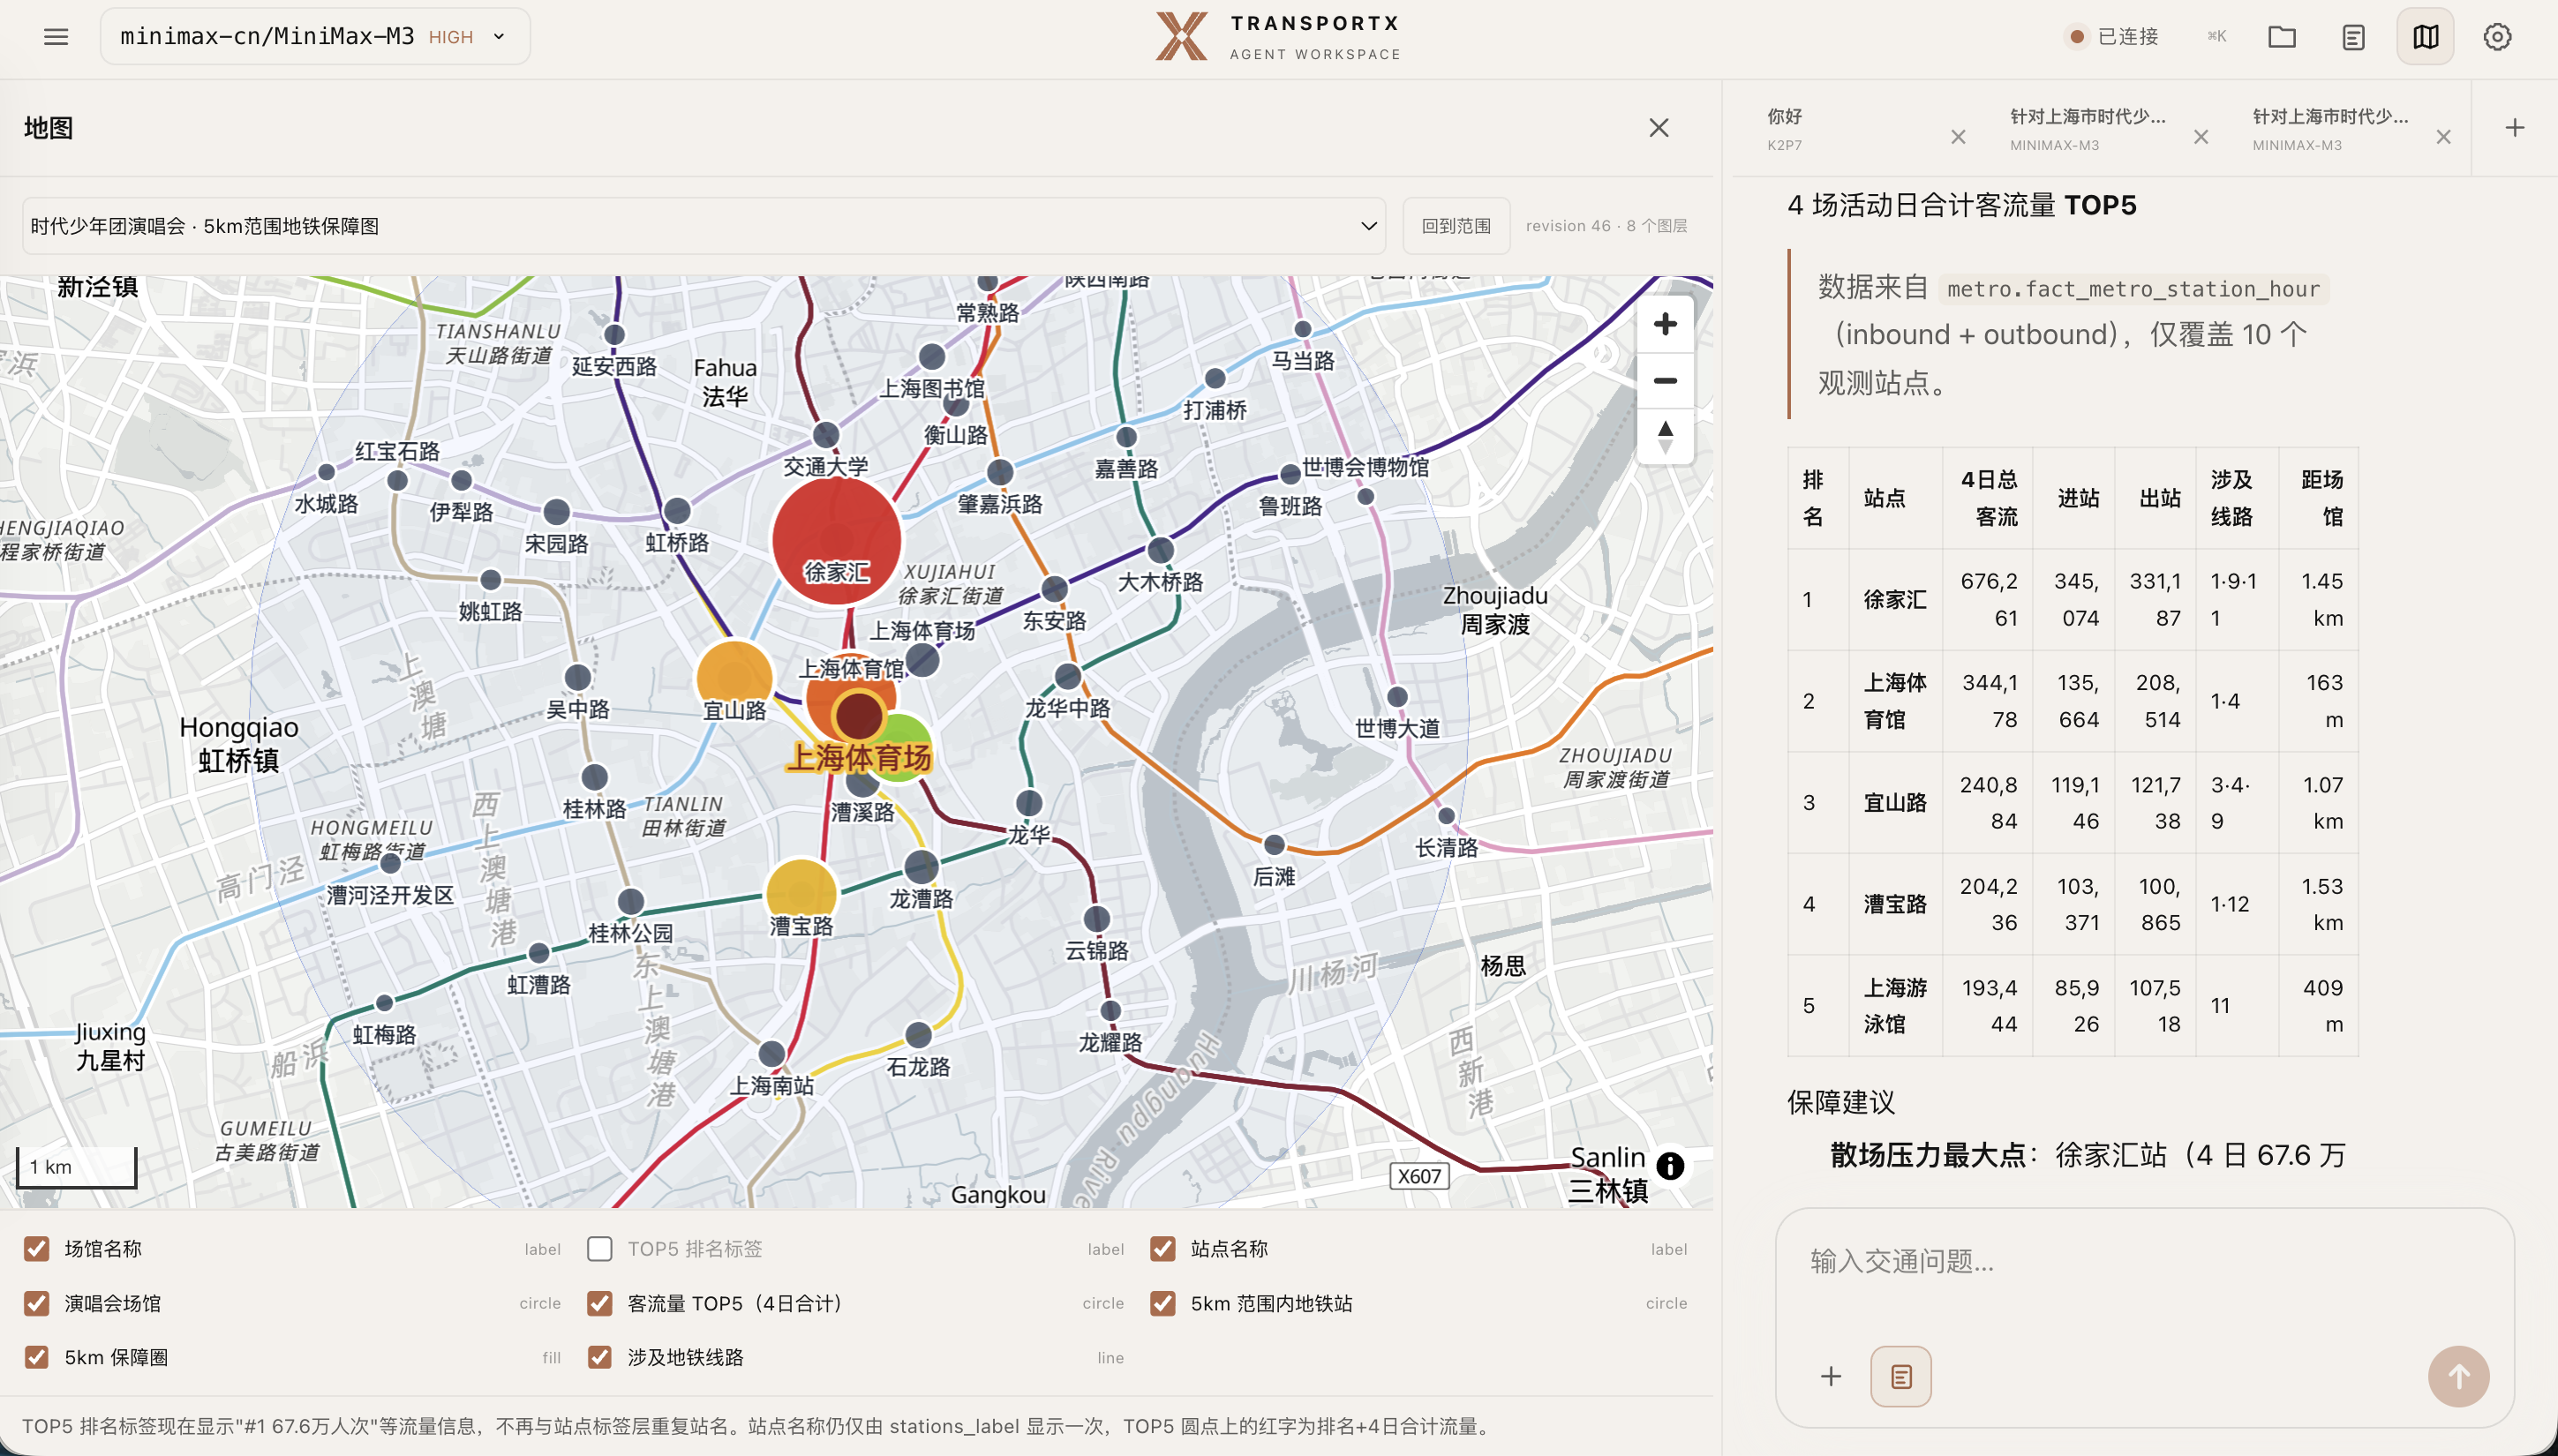
\includegraphics[width=0.92\linewidth]{02-metro-保障图.png}
  \caption{上海体育场 5 km 范围轨交保障图与四场活动日客流 TOP5}
  \label{fig:metro}
\end{figure}

轨交保障图以场馆为中心绘制 5 km 保障圈，叠加范围内站点、涉及线路和场馆标记，并在对话区同步给出四场活动日客流量 TOP5、进出站拆分、涉及线路和距场馆距离。图层面板允许分别控制场馆名称、保障圈、线路、站点和排名标记，便于从全局网络切换到重点站点核查。

\begin{figure}[ht]
  \centering
  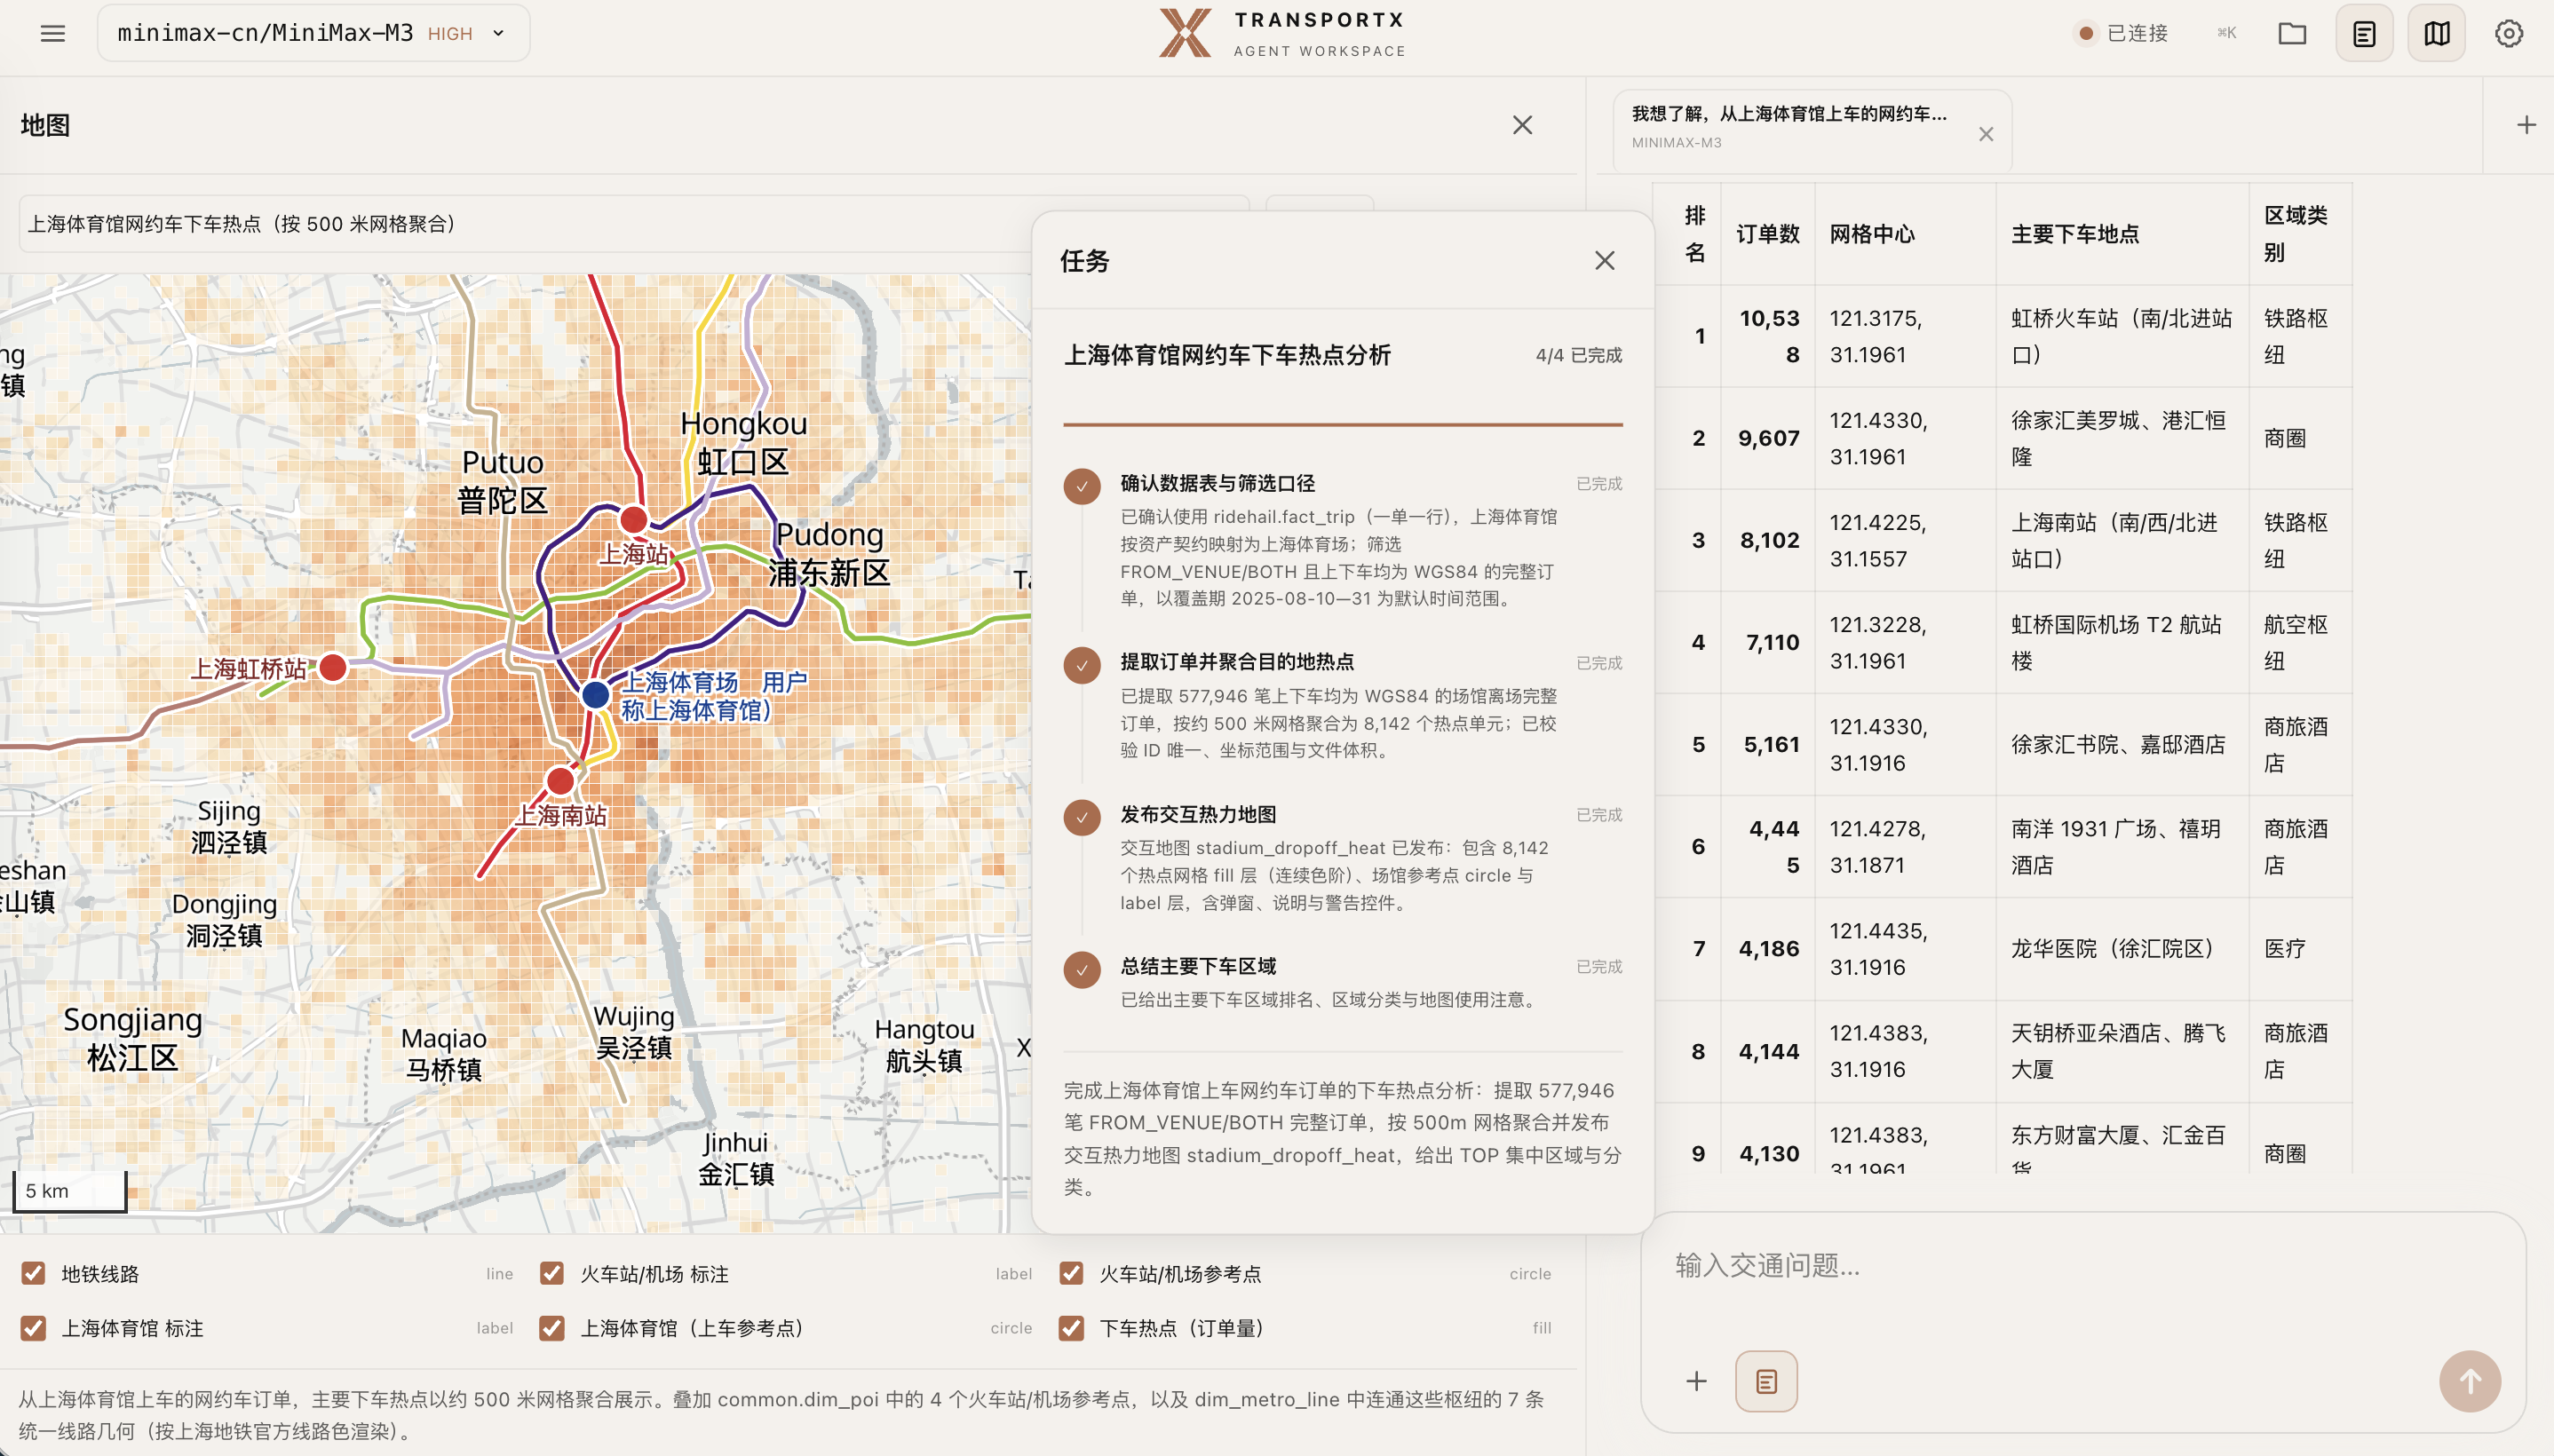
\includegraphics[width=0.92\linewidth]{03-ridehail-dropoff-heatmap.png}
  \caption{散场网约车下车热点、重要场站与轨交线路叠加分析}
  \label{fig:ridehail}
\end{figure}

网约车示例从场馆离场完整订单中提取下车端点，按约 500 m 网格聚合为热度图，并叠加上海体育场、火车站/机场参考点和相关轨交线路。任务看板同步记录数据表与筛选口径确认、订单提取与网格聚合、交互地图发布、主要下车区域总结四个步骤；右侧结果表给出热点网格排名、订单数、网格中心、主要下车地点和区域类别，使地图分布与统计结果可以相互校验。

\begin{figure}[ht]
  \centering
  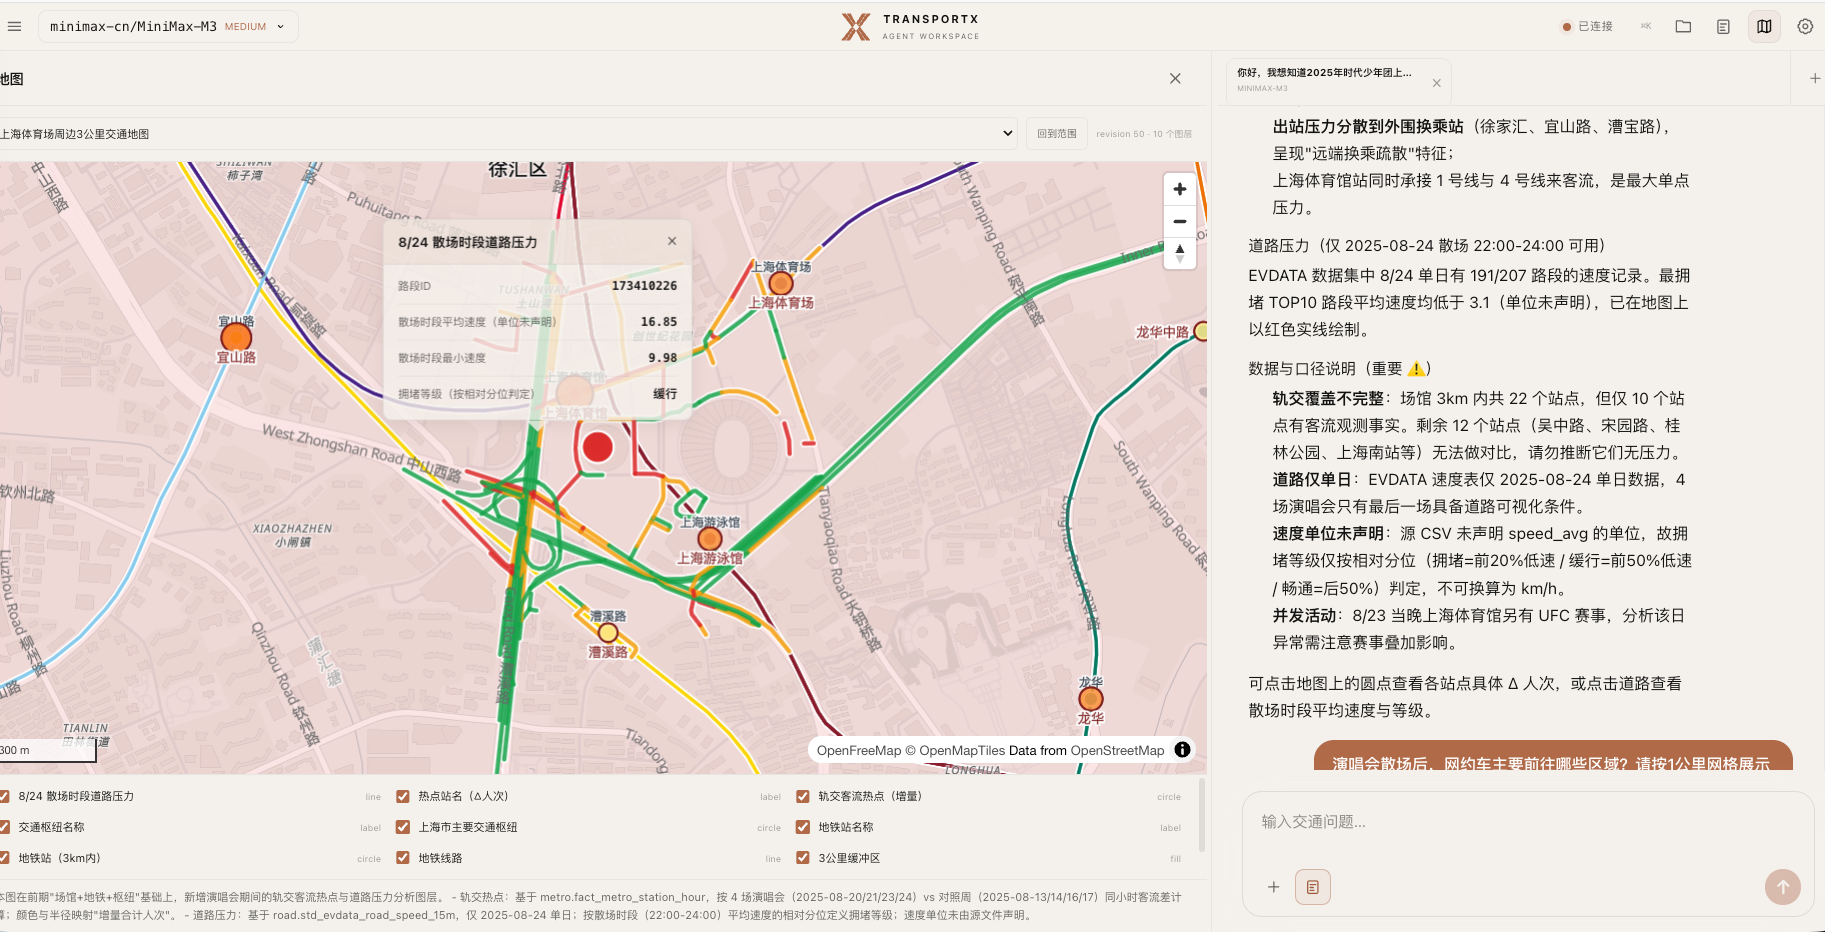
\includegraphics[width=0.92\linewidth]{06-evdata-road-pressure.png}
  \caption{散场时段道路压力专题图与站点点击详情（基于 EVDATA 数据）}
  \label{fig:evdata}
\end{figure}

EVDATA 图以 2025-08-24 散场 22:00--24:00 的 207 个场馆周边 WGS84 路段为样本，按平均速度与拥堵等级上色：红色为拥堵、绿色为缓行、灰色为畅通。图层叠加场馆周边 3 公里缓冲圈、轨交枢纽与重点商圈。点击地图上的站点或路段，右侧弹出当前对象的实时详情（如路段 ID、平均速度、最小速度、拥堵等级），并在对话区同步汇总 TOP10 拥堵路段与“轨交出入口压力分入外围换乘点”等研判结论。

\begin{figure}[ht]
  \centering
  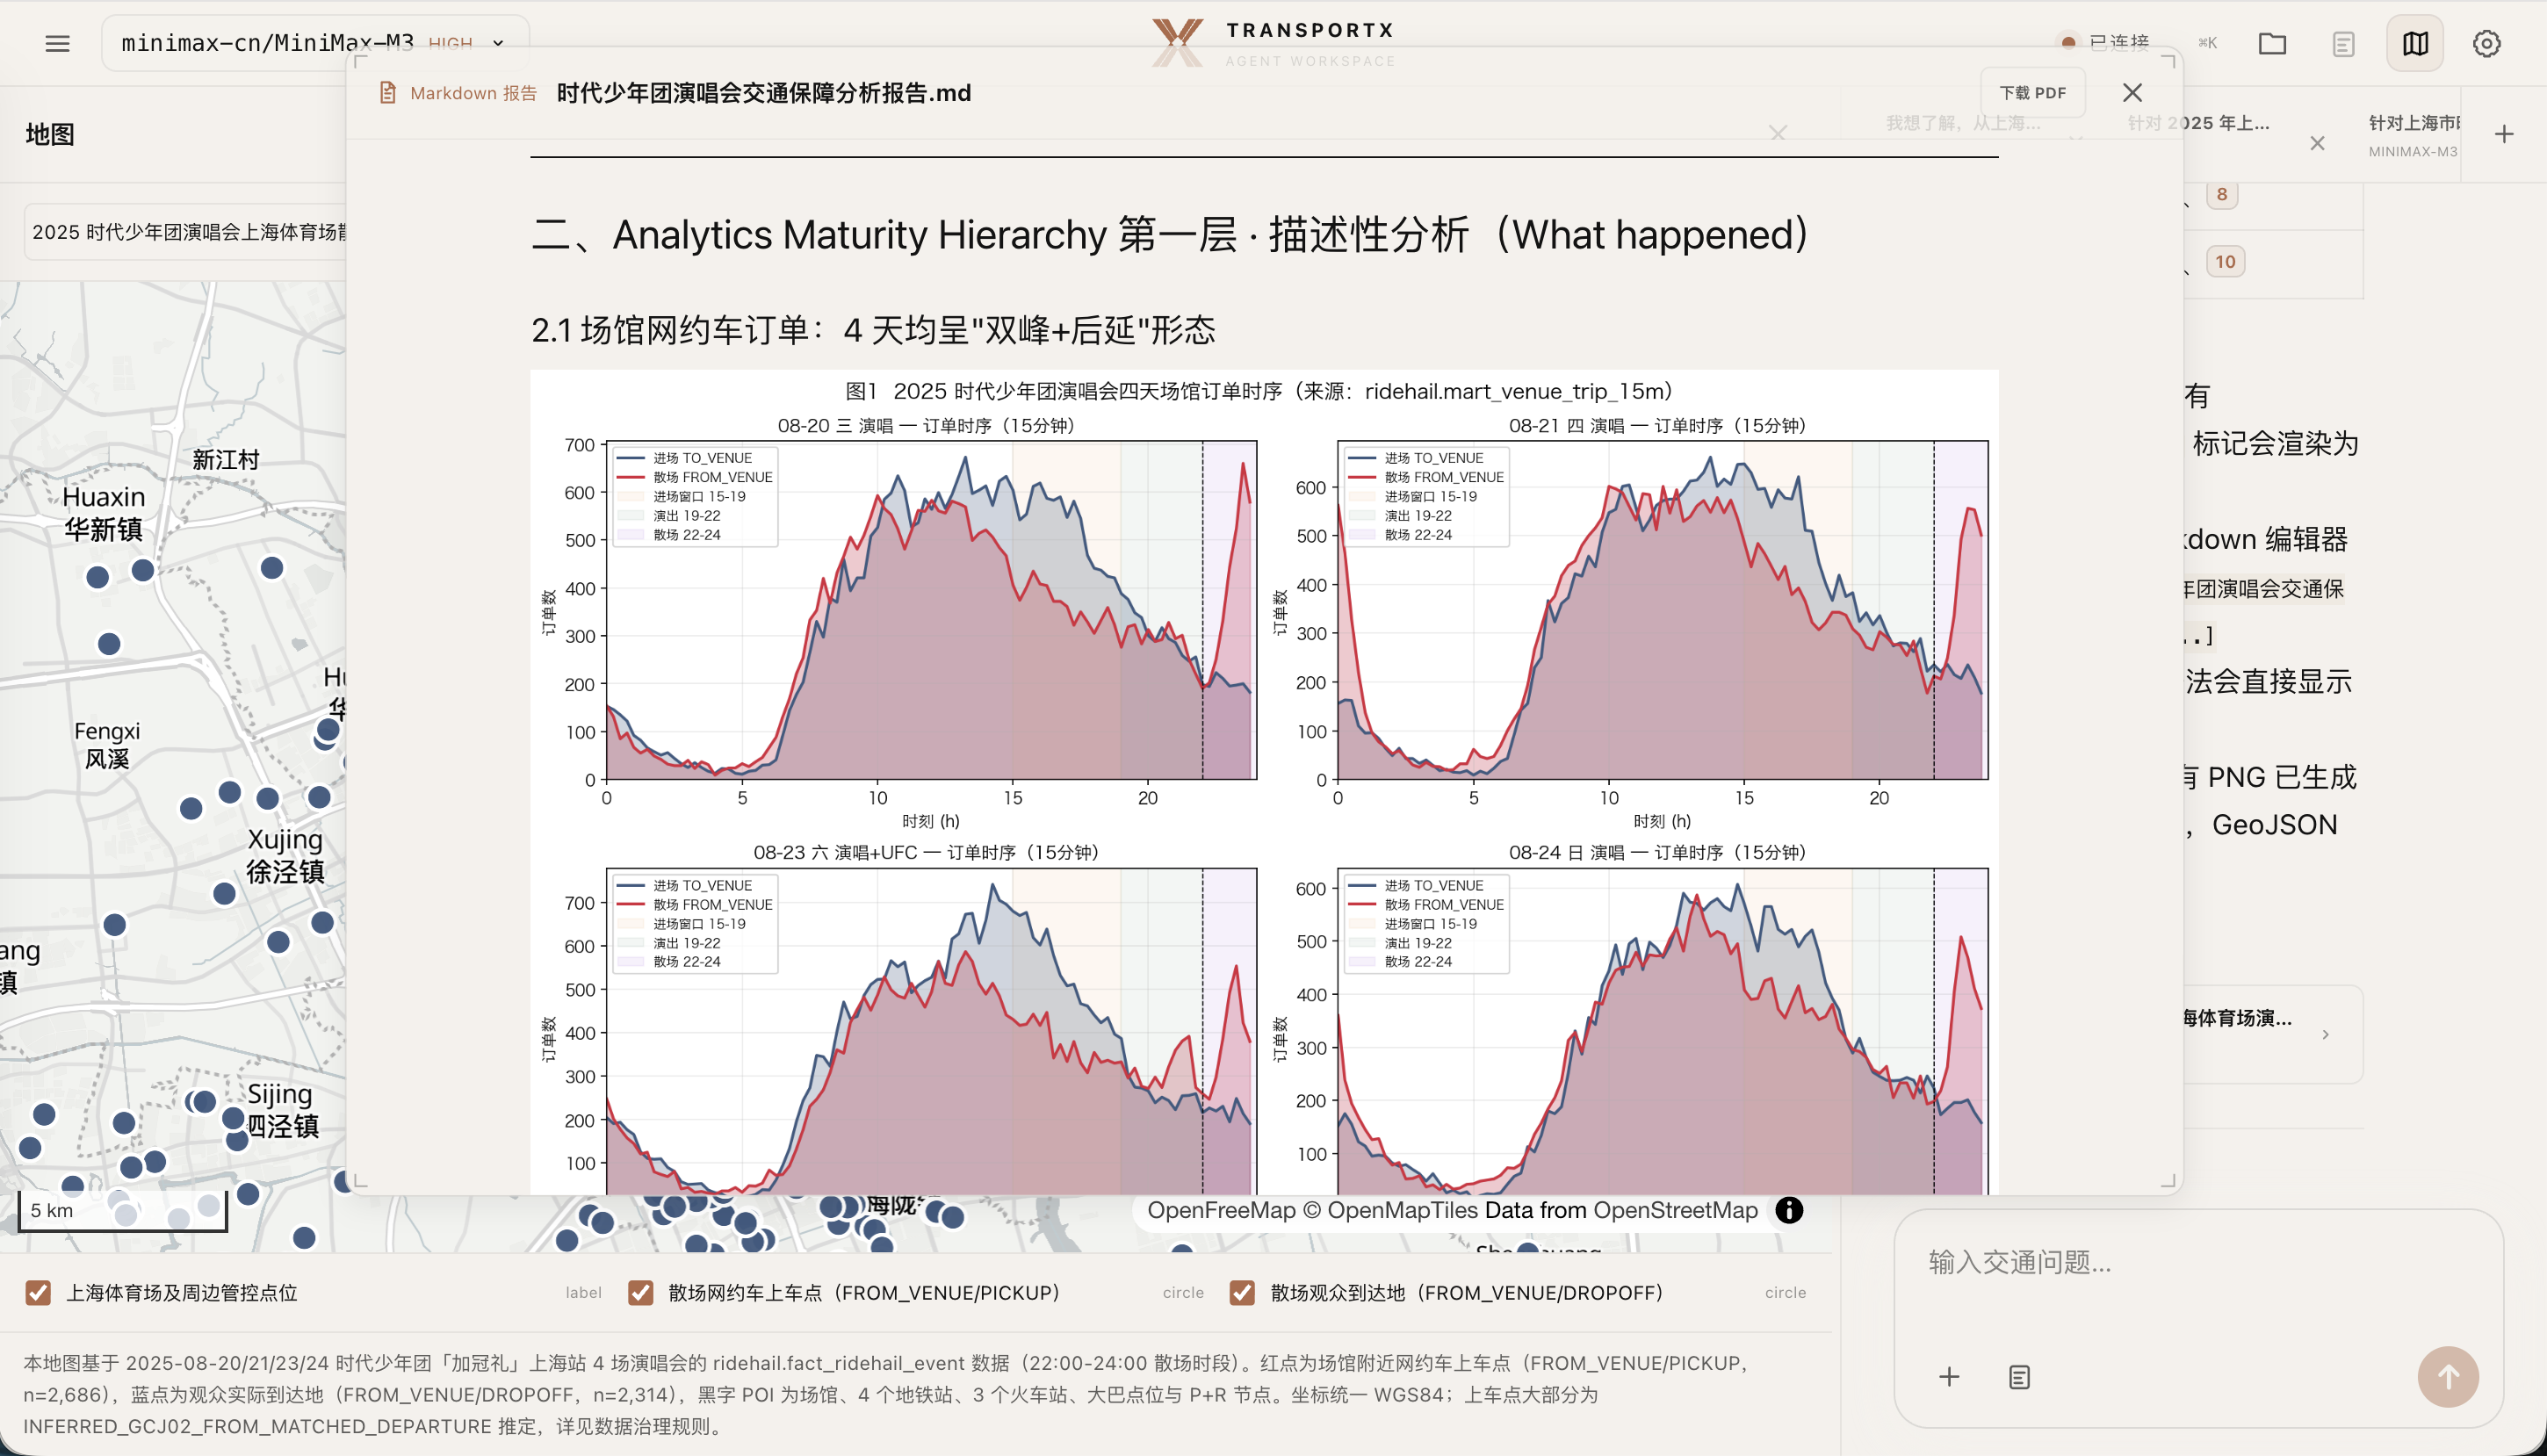
\includegraphics[width=0.92\linewidth]{04-report-preview.png}
  \caption{时代少年团演唱会交通保障分析报告预览}
  \label{fig:report}
\end{figure}

Markdown 报告预览将 15 分钟粒度的进场、散场订单曲线与分析文字放在同一版面，同时保留地图和会话上下文。用户可在工作台内检查图表、正文和分页效果，确认后下载 PDF。

\begin{figure}[ht]
  \centering
  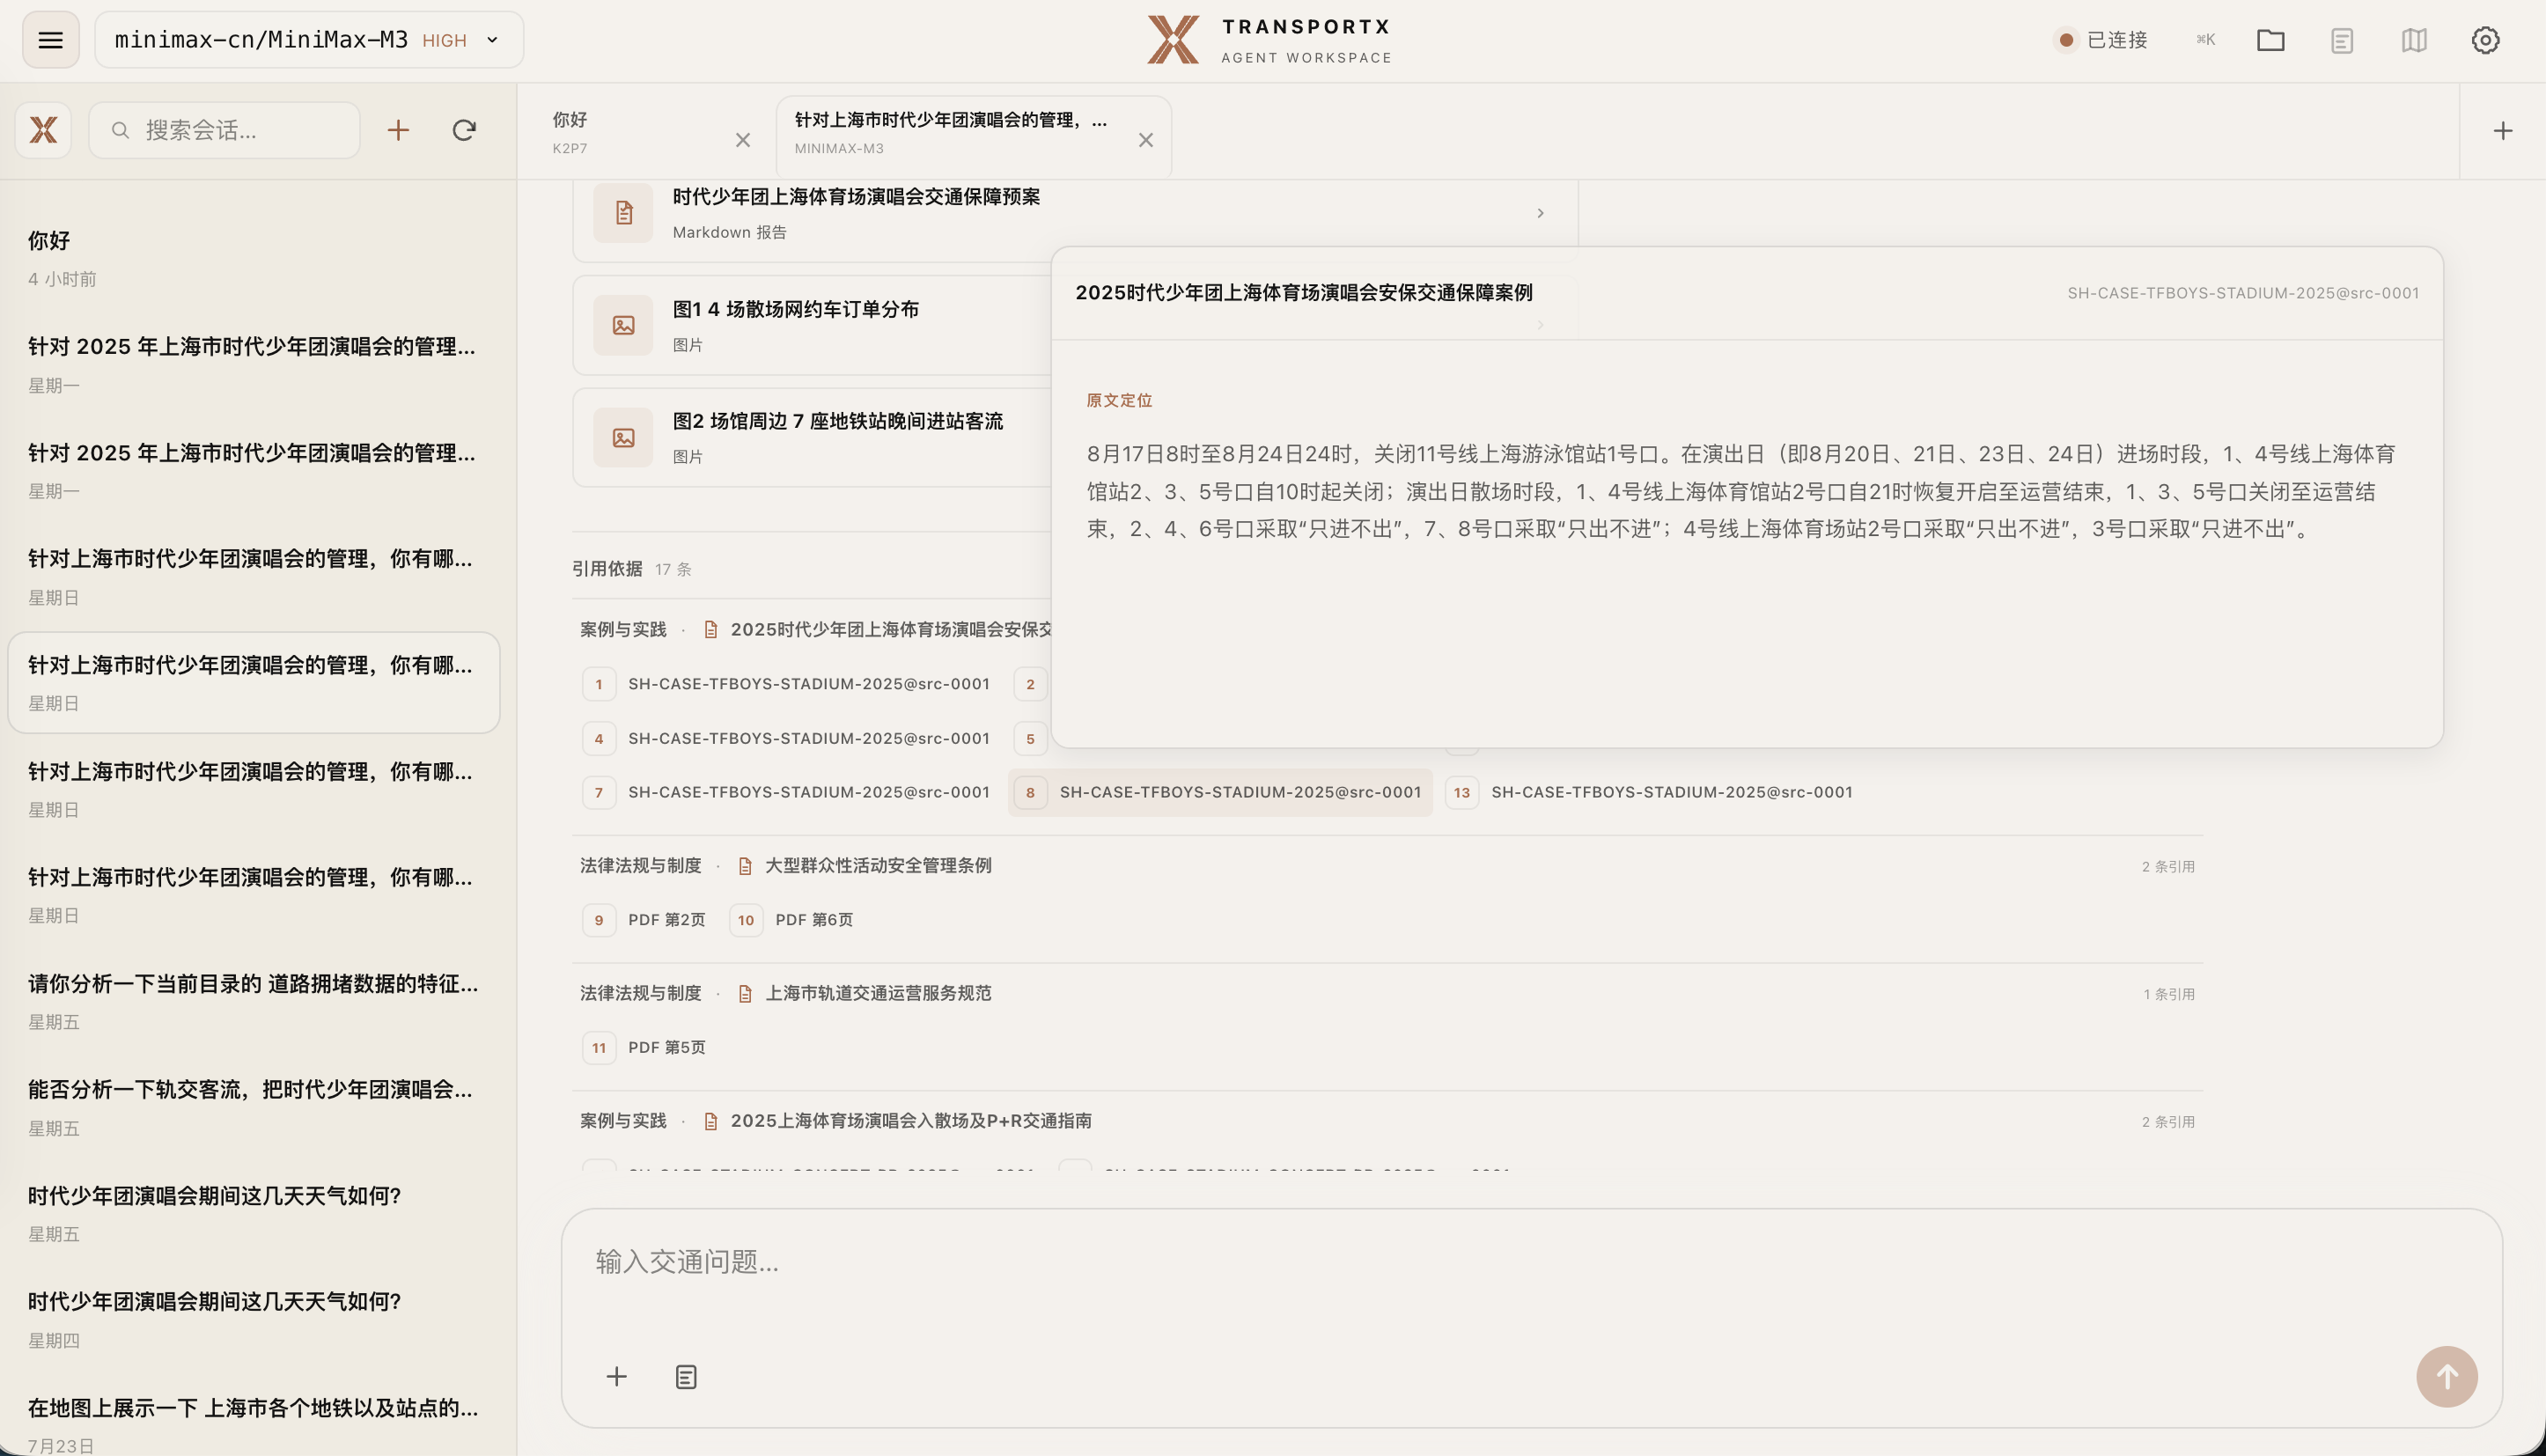
\includegraphics[width=0.92\linewidth]{05-citation-detail.png}
  \caption{交通保障案例的引用清单与原文定位}
  \label{fig:citation}
\end{figure}

引用区按知识类别和来源文档汇总本次报告实际使用的证据，并保留引用编号、知识 ID 和 PDF 页码。点击编号后，原文定位浮层直接展示对应段落，例如车站出入口调整、进出站组织等具体措施，从而支持``报告结论—引用条目—来源原文''的逐级复核。

地图数据先完成分析和校验，再发布到浏览器。\code{publish\_geodata} 检查 GeoJSON 的路径、大小、要素数、坐标和 ID，\code{present\_visualization} 执行白名单内的命令。浏览器复用同一 \code{visualizationId}，以增量方式添加图层或修改样式，并保留用户设置的图层显隐状态。

% =============================================================================
%  六、可拓展性与安全合规设计
% =============================================================================
\newpage
\section{可拓展性与安全合规设计}

\subsection{系统可拓展性设计}

分域数据、项目级 Skill 和共享契约承担扩展接口。接入新活动或数据源时，开发人员补充源数据登记、标准字段、质量规则、分域事实或集市以及参考文档，工作台主体保持不变。

\begin{enumerate}
  \item \term{新数据接入：}盘点源文件与许可证/使用范围 $\rightarrow$ 建立字段映射和 CRS/时区规则 $\rightarrow$ 写入标准层 $\rightarrow$ 生成事实与集市 $\rightarrow$ 运行质量断言 $\rightarrow$ 更新目录与 Skill。
  \item \term{跨场景迁移：}保留会话、任务、引用、地图和报告链路，替换活动维度、场馆 POI、数据资产和案例知识；不同项目继续使用独立任务目录。
  \item \term{模型升级：}RuntimeCapabilities 发布模型身份和 thinking 等能力；前端只读取共享契约。
  \item \term{能力升级：}新增工具通过 Extension 注册，通过版本化 Bridge 发布完整 Manifest；浏览器根据 capability 决定展示。
  \item \term{规模升级：}当前 GeoJSON 上限为 5 万要素/20 MiB；只有数据规模达到瓶颈时再引入 MVT/PMTiles 或独立检索服务。
\end{enumerate}

SQLite 和模块化单体适合当前的数据规模、本地部署方式和交付周期，也便于离线演示。多用户、高并发或实时流数据场景需要重新评估数据库、任务队列、权限中心和地图切片方案。

\subsection{数据安全与合规设计}

\begin{itemize}
  \item \term{数据最小化：}原始文件和数据库通过受控数据包管理，查询资产只保留分析所需字段。
  \item \term{查询权限：}数据库使用只读模式，并限制 SQL 类型、对象名称和返回行数，降低误写和批量导出风险。
  \item \term{隐私保护：}订单号经过 SHA-256 假名化，用于去重和关联；地点文本按敏感字段管理，默认输出聚合结果。
  \item \term{空间合规：}发布数据只使用 EPSG:4326 或标记为未知的坐标。精确空间分析只采用坐标系已经确认的记录，转换过程保留来源和质量状态。
  \item \term{会话隔离：}文件、空间数据和引用资源绑定任务会话，系统阻断跨会话读取和路径越界。
  \item \term{内容安全：}地图由结构化命令驱动，Markdown 和链接经过安全校验后再呈现。
  \item \term{访问控制：}系统通过签名 Cookie、同源 WebSocket 和资源鉴权控制访问，当前适用于本机或受控演示环境。
  \item \term{引用校验：}知识和任务产物登记真实路径及 SHA-256。原件缺失或内容变化时，界面显示异常状态。
\end{itemize}

\begin{warning}
局域网或多人试用版本需要配置强制身份认证、角色与数据域授权、访问审计、会话配额、断线命令恢复、密钥托管和备份恢复。敏感明细的导出范围由数据管理部门审批。
\end{warning}

\subsection{技术架构与关键边界}

下图给出系统从 Pi Extension 到 Node Server 再到 React Workspace 的三层架构、之间的传输协议，以及贯穿全栈的共享契约与安全边界，作为本节能力设计与合规要求的对应关系图。。

\begin{figure}[ht]
\centering
\begin{tikzpicture}[
  font=\small\sffamily,
  every node/.style={align=center},
  scale=0.92, transform shape,
  layer/.style={
    rectangle, rounded corners=3pt, draw=TipColor!70!black, very thick,
    fill=TipColor!6, inner sep=8pt
  },
  module/.style={
    rectangle, rounded corners=2pt, draw=black!55, fill=white,
    minimum height=8mm, inner sep=3pt, font=\footnotesize\sffamily,
    text width=23mm
  },
  group/.style={
    rectangle, rounded corners=2pt, draw=black!40, dashed,
    inner sep=4pt, fill=black!2
  },
  arr/.style={-{Stealth[length=2.4mm]}, thick, draw=black!70},
  label/.style={font=\scriptsize\sffamily, fill=white, inner sep=1pt}
]
% ================ 第 1 层：Pi Extension ================
\node[module] (ext1) {pi-task-mode};
\node[module, right=3mm of ext1] (ext2) {pi-geo-\\visualization};
\node[module, right=3mm of ext2] (ext3) {pi-citation};
\node[module, right=3mm of ext3] (ext4) {pi-web-bridge};
\begin{scope}[on background layer]
  \node[layer, fit=(ext1)(ext2)(ext3)(ext4)] (layer1) {};
\end{scope}
\node[above=2pt of layer1.north, font=\sffamily\bfseries\small]
  {Pi Extension Layer (Coding Agent)};

% ================ 第 2 层：Node Server ================
% 用相对定位表达 svMain 在 layer1 下方居中
\node[module, below=16mm of layer1.south, anchor=north,
      xshift=-30mm, text width=28mm, minimum height=11mm] (svMain)
  {server-main\\\scriptsize 认证 / RPC / 装配\\[-1pt]\scriptsize / CLI 生命周期};
\node[module, right=2mm of svMain, text width=24mm, minimum height=11mm] (svRoutes)
  {api-routes\\\scriptsize 类型化 HTTP\\[-1pt]\scriptsize 路由表};

\node[module, below=3mm of svMain, text width=28mm] (svHist)
  {session-history-handler\\\scriptsize JSONL 历史 / 搜索\\[-1pt]\scriptsize / 项目聚合};
\node[module, right=2mm of svHist, text width=24mm] (svFile)
  {file-api-handler\\\scriptsize 会话内文件 / 预览\\[-1pt]\scriptsize / 本机打开};

\node[module, below=3mm of svHist, text width=28mm] (svWs)
  {websocket-handler\\\scriptsize 同源升级 / 连接\\[-1pt]\scriptsize / 心跳};
\node[module, right=2mm of svWs, text width=24mm] (svCit)
  {citation-resources\\\scriptsize 引用原件\\[-1pt]\scriptsize 受控只读};
\node[module, right=2mm of svCit, text width=22mm] (svGeo)
  {geo-resources\\\scriptsize Geo 资源\\[-1pt]\scriptsize 会话路由};

\begin{scope}[on background layer]
  \node[layer, fit=(svMain)(svRoutes)(svHist)(svFile)(svWs)(svCit)(svGeo)] (layer2) {};
\end{scope}
\node[above=2pt of layer2.north, font=\sffamily\bfseries\small]
  {Node Server};

% ================ 第 3 层：React Workspace ================
\node[module, below=16mm of layer2.south, anchor=north,
      text width=42mm, minimum height=14mm] (brwKernel)
  {Browser Application Kernel\\\scriptsize Event normalizer / Command ports\\\scriptsize Stores: Runtime / Session /\\[-1pt]\scriptsize Conversation / Tool / Extension UI};

\node[module, below=3mm of brwKernel, xshift=-26mm, text width=27mm, minimum height=12mm] (brwPlat)
  {Platform\\\scriptsize 对话 / 会话 /\\[-1pt]\scriptsize 设置 / 文件预览};
\node[module, right=3mm of brwPlat, text width=27mm, minimum height=12mm] (brwFeat)
  {Features\\\scriptsize Citation / Task Board\\[-1pt]\scriptsize / lazy Geo Workspace};

\begin{scope}[on background layer]
  \node[layer, fit=(brwKernel)(brwPlat)(brwFeat)] (layer3) {};
\end{scope}
\node[above=2pt of layer3.north, font=\sffamily\bfseries\small]
  {React Workspace (Browser)};

% ================ 数据流箭头 ================
\draw[arr] ([yshift=-2mm]layer1.south) --
  node[midway, above=2pt, font=\scriptsize\sffamily, fill=white, inner sep=1pt]{JSONL / RPC}
  ([yshift=+2mm]layer2.north);
\draw[arr] ([yshift=-2mm]layer2.south) --
  node[midway, above=2pt, font=\scriptsize\sffamily, fill=white, inner sep=1pt]{HTTP / WebSocket（同源）}
  ([yshift=+2mm]layer3.north);

% ================ 底部：共享契约 + 安全边界 ================
\node[group, below=8mm of layer3.south, anchor=north,
      text width=150mm, inner sep=5pt] (contracts)
  {\sffamily\bfseries 共享契约 \texttt{src/contracts/}\\[1pt]
   \normalfont\sffamily\scriptsize SessionSnapshot · TaskSnapshot · GeoScene · Citation · Bridge · 诊断 · 版本
   \quad（契约不依赖 Node / React / DOM / MapLibre）};

\node[group, below=2mm of contracts.south, anchor=north,
      text width=150mm, inner sep=5pt] (boundary)
  {\sffamily\bfseries 安全边界\\[1pt]
   \normalfont\sffamily\scriptsize
   $\bullet$ 会话目录 = 权限边界（路径越界、符号链接越界、跨会话读取拒绝）
   \quad $\bullet$ 数据库只读（限制 SQL 类型 / 对象名 / 返回行数）\\[1pt]
   $\bullet$ 同源 WebSocket（签名 Cookie + 资源鉴权）
   \quad $\bullet$ 引用原件受控只读（SHA-256 摘要校验 + 会话隔离）};
\end{tikzpicture}
\caption{技术架构与关键边界（Pi Extension → Node Server → React Workspace）}
\label{fig:tech-arch}
\end{figure}

% \subsection{可扩展的若干演进路径} ← 如需保留可手动解开

% =============================================================================
%  七、结果展示
% =============================================================================

% =============================================================================
%  七、结果展示
% =============================================================================
\newpage
\section{结果展示}

\subsection{核心能力量化测试结果}

本节记录自动化测试结果和可复核的资产规模。工程测试覆盖运行链路、协议和安全边界。业务问数准确率与方案采纳率另行验收。

\begin{table}[ht]
  \centering
  \caption{核心能力量化测试结果}
  \label{tab:tests}
  \begin{tabularx}{\linewidth}{@{}lcX@{}}
    \toprule
    \rowcolor{TableHead}
    \sffamily\bfseries 验证项 & \sffamily\bfseries 结果 & \sffamily\bfseries 范围/说明 \\
    \midrule
    项目构建      & 通过    & 服务端、前端和地图模块 \\
    自动化测试    & 70/70 通过 & 会话、鉴权、任务、地图和引用 \\
    浏览器冒烟    & 通过    & 桌面端和移动端关键交互 \\
    数据质量规则  & 错误级全部通过 & 唯一性、坐标和集市加和关系 \\
    知识库索引    & 38 份文档 & 3,828 个节点、3,363 条知识项 \\
    业务准确率    & 待验收  & 需建立专家标注题集 \\
    \bottomrule
  \end{tabularx}
\end{table}

下一阶段计划建立不少于 100 道分层问数题和 10--20 个完整保障场景，交由交通业务、数据和安全人员分别评分。问数题覆盖口径辨析、单表、多表、时间窗口、空间条件和异常输入。方案评估记录事实正确性、依据有效性、措施可执行性、风险遗漏和人工改写量。

\subsection{业务场景效果验证}

\begin{itemize}
  \item \term{上海体育场周边轨交网络：}筛选场馆 5 km 范围内的站点，叠加线路、站点、场馆标签和活动日客流排名。验证内容包括坐标投影、线路颜色、站点数量、排名口径和图层可读性。
  \item \term{网约车需求热度：}按约 500 m 网格汇总下车端点，并叠加上海体育场、重要交通枢纽和轨交线路。结果使用聚合数据，同时说明热点口径和坐标状态。
  \item \term{活动日多方式趋势：}按照演前、演中和散场时段，对比网约车、公交、轨交、组织方道路状态和 EVDATA 道路速度。各交通方式分开标注单位，只比较共同覆盖日期。
  \item \term{散场道路压力专题：}基于 EVDATA 2025-08-24 散场 22:00--24:00 的 207 个场馆周边路段与 14977 条 15 分钟速度记录，绘制散场路网压力专题图，汇总 TOP10 拥堵路段、平均速度、拥堵等级与口径说明。点击地图上的站点或路段，弹出实时详情，并在对话区同步输出“为什么该路段拥堵”“场馆周边与外围换乘点的压力转移”类研判结论。
  \item \term{知识辅助方案：}从法规、标准、预案和案例中定位相关条款，生成带来源的建议。引用内容按法律义务、标准要求、预案程序和案例经验分别说明。
  \item \term{报告交付：}将对话结论、引用、图片和数据文件汇总为 Markdown 报告，支持在线预览和 PDF 导出。参考依据只收录正文实际使用的来源。
\end{itemize}

现有演示已在同一任务中完成数据查询、空间叠加、过程说明和成果文件生成。当前验证结论为系统链路可运行、结果可复核。生产指挥准确率需通过独立业务盲测确定。

\subsection{已知缺陷与边界说明}

\begin{itemize}
  \item \term{数据时间跨度：}各事实域约 21--22 天，适用于活动期短周期对比。年度规律、节假日模型和长期预测需要补充长期数据。
  \item \term{空间覆盖：}轨交客流覆盖 10 个物理站；原 89 个道路发布段没有几何；EVDATA 已入库 2025-08-24 的 207 个场馆周边路段样本，路段映射待建立；天气网格 CRS 待确认。
  \item \term{样本范围：}订单、公交和道路数据以徐汇区及场馆相关样本为主，结论适用于当前样本范围。
  \item \term{业务验收：}专家标注的问数题库和方案评分集待建立，准确率和采纳率将在盲测后填写。
  \item \term{部署范围：}当前版本适合本机或受控演示。多人和局域网部署需要增加认证、授权、审计与配额。
  \item \term{数据库安装：}Git checkout 包含代码、Skill、参考文档和脚本，交通数据库由受控安装包提供。查询功能在数据库安装后启用。
  \item \term{决策责任：}交通管理、运营、公安和活动承办单位按职责核实并批准系统建议。
\end{itemize}

% =============================================================================
%  八、成果交付清单
% =============================================================================
\newpage
\section{成果交付清单}

\subsection{文档类交付物}

\begin{itemize}
  \item \term{项目建设说明报告：}本文件，编制日期为 2026 年 7 月 30 日。报告说明项目建设内容和验收边界，后续更新以本文件为准。
  \item \code{README.md}：版本 v2.14.0，说明产品能力、启动方式、验证命令和运行约束。
  \item \term{系统架构说明}（\code{docs/ARCHITECTURE.md}）：说明系统边界、依赖方向和各模块职责。
  \item \term{可信引用技术方案}（\code{docs/CITATION\_FEATURE\_TECHNICAL\_PLAN.md}）：记录引用机制、报告产物和验收情况。
  \item \term{测试基线}（\code{docs/TEST\_BASELINES.md}）：记录默认测试和浏览器验证范围。
  \item \term{版本变更记录}（\code{docs/CHANGELOG.md}）：记录截至 v2.14 的版本演进和验证结果。
  \item \term{数据资产说明与审查记录}（\code{docs/skills/shanghai-traffic-data-assets-*.md}）：版本 3.1.0，说明数据覆盖、字段结构、指标口径、空间信息、EVDATA 接入和治理结果。
\end{itemize}

\subsection{系统类交付物}

\begin{itemize}
  \item 交通态势智能工作台 v2.14.0 源码与构建脚本：Node/TypeScript 服务、React 工作台、浏览器 Kernel 和共享契约。
  \item Task Mode、Geo Visualization、Citation、Web Bridge 等扩展组件。
  \item shanghai-traffic-data-assets、search-traffic-assurance-knowledge、geo-visualization-explanation、plot-from-data 等项目级 Skill；结构化知识目录和原件由独立 Knowledge Module 提供，不与检索 Skill 捆绑。
  \item 自动化测试、浏览器冒烟、真实运行时 RPC 冒烟和测试夹具。
  \item 受控数据安装包：6 个 SQLite 分域库及查询/治理脚本；数据库与原始数据单独交付。
\end{itemize}

\begin{tip}
在项目目录执行 \code{npm install} 后运行 \code{./start.sh}，默认访问 \code{http://127.0.0.1:3000}。也可先执行 \code{npm run build}，再用 \code{node bin/tau.js --host 127.0.0.1 --port 3001 --open} 启动。服务使用当前用户权限。受控数据库、密钥和原始数据按部署环境单独配置。
\end{tip}

\subsection{其他配套交付物}

仓库提供首页、设置、命令面板、移动端和交通地图分析截图，可直接用于汇报。地图示例包括上海体育场周边轨交网络、网约车热度与重要场站叠加。演示视频可按``新建交通任务—开启任务模式—完成问数—生成地图—导出报告''的路径录制。

交通数据库和组织方原始交通数据通过受控安装包交付。代码仓库可独立启动界面，安装数据库后开放数据查询。法规、标准、预案和案例的原件及结构化索引由独立 Knowledge Module 安装，运行时再与知识检索 Skill 装配。

\end{document}
